\documentclass[twoside]{book}

% Packages required by doxygen
\usepackage{fixltx2e}
\usepackage{calc}
\usepackage{doxygen}
\usepackage[export]{adjustbox} % also loads graphicx
\usepackage{graphicx}
\usepackage[utf8]{inputenc}
\usepackage{makeidx}
\usepackage{multicol}
\usepackage{multirow}
\PassOptionsToPackage{warn}{textcomp}
\usepackage{textcomp}
\usepackage[nointegrals]{wasysym}
\usepackage[table]{xcolor}

% Font selection
\usepackage[T1]{fontenc}
\usepackage[scaled=.90]{helvet}
\usepackage{courier}
\usepackage{amssymb}
\usepackage{sectsty}
\renewcommand{\familydefault}{\sfdefault}
\allsectionsfont{%
  \fontseries{bc}\selectfont%
  \color{darkgray}%
}
\renewcommand{\DoxyLabelFont}{%
  \fontseries{bc}\selectfont%
  \color{darkgray}%
}
\newcommand{\+}{\discretionary{\mbox{\scriptsize$\hookleftarrow$}}{}{}}

% Page & text layout
\usepackage{geometry}
\geometry{%
  a4paper,%
  top=2.5cm,%
  bottom=2.5cm,%
  left=2.5cm,%
  right=2.5cm%
}
\tolerance=750
\hfuzz=15pt
\hbadness=750
\setlength{\emergencystretch}{15pt}
\setlength{\parindent}{0cm}
\setlength{\parskip}{3ex plus 2ex minus 2ex}
\makeatletter
\renewcommand{\paragraph}{%
  \@startsection{paragraph}{4}{0ex}{-1.0ex}{1.0ex}{%
    \normalfont\normalsize\bfseries\SS@parafont%
  }%
}
\renewcommand{\subparagraph}{%
  \@startsection{subparagraph}{5}{0ex}{-1.0ex}{1.0ex}{%
    \normalfont\normalsize\bfseries\SS@subparafont%
  }%
}
\makeatother

% Headers & footers
\usepackage{fancyhdr}
\pagestyle{fancyplain}
\fancyhead[LE]{\fancyplain{}{\bfseries\thepage}}
\fancyhead[CE]{\fancyplain{}{}}
\fancyhead[RE]{\fancyplain{}{\bfseries\leftmark}}
\fancyhead[LO]{\fancyplain{}{\bfseries\rightmark}}
\fancyhead[CO]{\fancyplain{}{}}
\fancyhead[RO]{\fancyplain{}{\bfseries\thepage}}
\fancyfoot[LE]{\fancyplain{}{}}
\fancyfoot[CE]{\fancyplain{}{}}
\fancyfoot[RE]{\fancyplain{}{\bfseries\scriptsize Generated by Doxygen }}
\fancyfoot[LO]{\fancyplain{}{\bfseries\scriptsize Generated by Doxygen }}
\fancyfoot[CO]{\fancyplain{}{}}
\fancyfoot[RO]{\fancyplain{}{}}
\renewcommand{\footrulewidth}{0.4pt}
\renewcommand{\chaptermark}[1]{%
  \markboth{#1}{}%
}
\renewcommand{\sectionmark}[1]{%
  \markright{\thesection\ #1}%
}

% Indices & bibliography
\usepackage{natbib}
\usepackage[titles]{tocloft}
\setcounter{tocdepth}{3}
\setcounter{secnumdepth}{5}
\makeindex

% Custom commands
\newcommand{\clearemptydoublepage}{%
  \newpage{\pagestyle{empty}\cleardoublepage}%
}

\usepackage{caption}
\captionsetup{labelsep=space,justification=centering,font={bf},singlelinecheck=off,skip=4pt,position=top}

%===== C O N T E N T S =====

\begin{document}

% Titlepage & ToC
\pagenumbering{alph}
\begin{titlepage}
\vspace*{7cm}
\begin{center}%
{\Large Segmented Fusion \\[1ex]\large v0.\+7 }\\
\vspace*{1cm}
{\large Generated by Doxygen 1.8.13}\\
\end{center}
\end{titlepage}
\clearemptydoublepage
\pagenumbering{roman}
\tableofcontents
\clearemptydoublepage
\pagenumbering{arabic}

%--- Begin generated contents ---
\chapter{Namespace Index}
\section{Namespace List}
Here is a list of all documented namespaces with brief descriptions\+:\begin{DoxyCompactList}
\item\contentsline{section}{\textbf{ Application} }{\pageref{namespace_application}}{}
\item\contentsline{section}{\textbf{ Body\+Parts} }{\pageref{namespace_body_parts}}{}
\item\contentsline{section}{\textbf{ dynamic\+Fusion} }{\pageref{namespacedynamic_fusion}}{}
\item\contentsline{section}{\textbf{ General} }{\pageref{namespace_general}}{}
\item\contentsline{section}{\textbf{ Menu} }{\pageref{namespace_menu}}{}
\item\contentsline{section}{\textbf{ R\+G\+BD} }{\pageref{namespace_r_g_b_d}}{}
\item\contentsline{section}{\textbf{ segmentation} }{\pageref{namespacesegmentation}}{}
\end{DoxyCompactList}

\chapter{Hierarchical Index}
\section{Class Hierarchy}
This inheritance list is sorted roughly, but not completely, alphabetically\+:\begin{DoxyCompactList}
\item \contentsline{section}{Body\+Parts.\+Body\+Parts}{\pageref{class_body_parts_1_1_body_parts}}{}
\item Frame\begin{DoxyCompactList}
\item \contentsline{section}{Application.\+Application}{\pageref{class_application_1_1_application}}{}
\item \contentsline{section}{Menu.\+Menu}{\pageref{class_menu_1_1_menu}}{}
\end{DoxyCompactList}
\item \contentsline{section}{G\+P\+U\+Manager.\+G\+P\+U\+Manager}{\pageref{class_g_p_u_manager_1_1_g_p_u_manager}}{}
\item \contentsline{section}{My\+\_\+\+Marching\+Cube.\+My\+\_\+\+Marching\+Cube}{\pageref{class_my___marching_cube_1_1_my___marching_cube}}{}
\item object\begin{DoxyCompactList}
\item \contentsline{section}{segmentation.\+Segmentation}{\pageref{classsegmentation_1_1_segmentation}}{}
\end{DoxyCompactList}
\item \contentsline{section}{R\+G\+B\+D.\+R\+G\+BD}{\pageref{class_r_g_b_d_1_1_r_g_b_d}}{}
\item \contentsline{section}{Stitching.\+Stitch}{\pageref{class_stitching_1_1_stitch}}{}
\item \contentsline{section}{tracking.\+Tracker}{\pageref{classtracking_1_1_tracker}}{}
\item \contentsline{section}{T\+S\+D\+F.\+T\+S\+D\+F\+Manager}{\pageref{class_t_s_d_f_1_1_t_s_d_f_manager}}{}
\end{DoxyCompactList}

\chapter{Class Index}
\section{Class List}
Here are the classes, structs, unions and interfaces with brief descriptions\+:\begin{DoxyCompactList}
\item\contentsline{section}{\textbf{ Application.\+Application} }{\pageref{class_application_1_1_application}}{}
\item\contentsline{section}{\textbf{ Body\+Parts.\+Body\+Parts} }{\pageref{class_body_parts_1_1_body_parts}}{}
\item\contentsline{section}{\textbf{ G\+P\+U\+Manager.\+G\+P\+U\+Manager} }{\pageref{class_g_p_u_manager_1_1_g_p_u_manager}}{}
\item\contentsline{section}{\textbf{ Menu.\+Menu} }{\pageref{class_menu_1_1_menu}}{}
\item\contentsline{section}{\textbf{ My\+\_\+\+Marching\+Cube.\+My\+\_\+\+Marching\+Cube} }{\pageref{class_my___marching_cube_1_1_my___marching_cube}}{}
\item\contentsline{section}{\textbf{ R\+G\+B\+D.\+R\+G\+BD} }{\pageref{class_r_g_b_d_1_1_r_g_b_d}}{}
\item\contentsline{section}{\textbf{ segmentation.\+Segmentation} }{\pageref{classsegmentation_1_1_segmentation}}{}
\item\contentsline{section}{\textbf{ Stitching.\+Stitch} }{\pageref{class_stitching_1_1_stitch}}{}
\item\contentsline{section}{\textbf{ tracking.\+Tracker} }{\pageref{classtracking_1_1_tracker}}{}
\item\contentsline{section}{\textbf{ T\+S\+D\+F.\+T\+S\+D\+F\+Manager} }{\pageref{class_t_s_d_f_1_1_t_s_d_f_manager}}{}
\end{DoxyCompactList}

\chapter{Namespace Documentation}
\section{Application Namespace Reference}
\label{namespace_application}\index{Application@{Application}}
\subsection*{Classes}
\begin{DoxyCompactItemize}
\item 
class \textbf{ Application}
\end{DoxyCompactItemize}
\subsection*{Variables}
\begin{DoxyCompactItemize}
\item 
\mbox{\label{namespace_application_a2fbdda0410c38b56264f744c6908835f}} 
{\bfseries R\+G\+BD} = imp.\+load\+\_\+source(\textquotesingle{}R\+G\+BD\textquotesingle{}, \textquotesingle{}./lib/R\+G\+B\+D.\+py\textquotesingle{})
\item 
\mbox{\label{namespace_application_a504993c7a678a17fdbb69a96ad9fef6a}} 
{\bfseries Track\+Manager} = imp.\+load\+\_\+source(\textquotesingle{}Track\+Manager\textquotesingle{}, \textquotesingle{}./lib/tracking.\+py\textquotesingle{})
\item 
\mbox{\label{namespace_application_abfb5c07a5ff0183031a6bfbd0993b799}} 
{\bfseries T\+S\+D\+Ftk} = imp.\+load\+\_\+source(\textquotesingle{}T\+S\+D\+Ftk\textquotesingle{}, \textquotesingle{}./lib/T\+S\+D\+F.\+py\textquotesingle{})
\item 
\mbox{\label{namespace_application_ac45436a85e7dd911ff145a77e6351ef7}} 
{\bfseries G\+PU} = imp.\+load\+\_\+source(\textquotesingle{}G\+P\+U\+Manager\textquotesingle{}, \textquotesingle{}./lib/G\+P\+U\+Manager.\+py\textquotesingle{})
\item 
\mbox{\label{namespace_application_a47a0bc7f73457e9921c018340281cda4}} 
{\bfseries My\+\_\+\+MC} = imp.\+load\+\_\+source(\textquotesingle{}My\+\_\+\+Marching\+Cube\textquotesingle{}, \textquotesingle{}./lib/My\+\_\+\+Marching\+Cube.\+py\textquotesingle{})
\item 
\mbox{\label{namespace_application_a4018729b4cf7db423a9d89e4346c7b92}} 
{\bfseries Stitcher} = imp.\+load\+\_\+source(\textquotesingle{}Stitcher\textquotesingle{}, \textquotesingle{}./lib/Stitching.\+py\textquotesingle{})
\item 
\mbox{\label{namespace_application_aeb29430194fcd06cda11b9f56fb432cd}} 
{\bfseries Bdy\+Prt} = imp.\+load\+\_\+source(\textquotesingle{}Body\+Parts\textquotesingle{}, \textquotesingle{}./lib/Body\+Parts.\+py\textquotesingle{})
\item 
\mbox{\label{namespace_application_a6f9414b74b3dea7e1b3ede67f9ff5d0b}} 
{\bfseries General} = imp.\+load\+\_\+source(\textquotesingle{}General\textquotesingle{}, \textquotesingle{}./lib/General.\+py\textquotesingle{})
\end{DoxyCompactItemize}


\subsection{Detailed Description}
\begin{DoxyVerb}File to handle program main loop
\end{DoxyVerb}
 
\hypertarget{namespace_body_parts}{}\section{Body\+Parts Namespace Reference}
\label{namespace_body_parts}\index{Body\+Parts@{Body\+Parts}}
\subsection*{Classes}
\begin{DoxyCompactItemize}
\item 
class \hyperlink{class_body_parts_1_1_body_parts}{Body\+Parts}
\end{DoxyCompactItemize}
\subsection*{Variables}
\begin{DoxyCompactItemize}
\item 
\mbox{\Hypertarget{namespace_body_parts_a1ab698cf581ff3eb738d64017cb23710}\label{namespace_body_parts_a1ab698cf581ff3eb738d64017cb23710}} 
{\bfseries PI} = math.\+pi
\item 
\mbox{\Hypertarget{namespace_body_parts_ad3cd6431ffd8e5ec138606939797bc27}\label{namespace_body_parts_ad3cd6431ffd8e5ec138606939797bc27}} 
{\bfseries R\+G\+BD} = imp.\+load\+\_\+source(\textquotesingle{}R\+G\+BD\textquotesingle{}, \textquotesingle{}./lib/R\+G\+B\+D.\+py\textquotesingle{})
\item 
\mbox{\Hypertarget{namespace_body_parts_aedf6f63744d6b69484e16917c5cb01af}\label{namespace_body_parts_aedf6f63744d6b69484e16917c5cb01af}} 
{\bfseries Track\+Manager} = imp.\+load\+\_\+source(\textquotesingle{}Track\+Manager\textquotesingle{}, \textquotesingle{}./lib/tracking.\+py\textquotesingle{})
\item 
\mbox{\Hypertarget{namespace_body_parts_a0a616cd1ce4a62524bf5d9d748c85f2b}\label{namespace_body_parts_a0a616cd1ce4a62524bf5d9d748c85f2b}} 
{\bfseries T\+S\+D\+Ftk} = imp.\+load\+\_\+source(\textquotesingle{}T\+S\+D\+Ftk\textquotesingle{}, \textquotesingle{}./lib/T\+S\+D\+F.\+py\textquotesingle{})
\item 
\mbox{\Hypertarget{namespace_body_parts_ab2dda25c9906c074315d122cef6f94bd}\label{namespace_body_parts_ab2dda25c9906c074315d122cef6f94bd}} 
{\bfseries G\+PU} = imp.\+load\+\_\+source(\textquotesingle{}G\+P\+U\+Manager\textquotesingle{}, \textquotesingle{}./lib/G\+P\+U\+Manager.\+py\textquotesingle{})
\item 
\mbox{\Hypertarget{namespace_body_parts_a6ee768ac808c89ad55a704afe5b4c8b5}\label{namespace_body_parts_a6ee768ac808c89ad55a704afe5b4c8b5}} 
{\bfseries My\+\_\+\+MC} = imp.\+load\+\_\+source(\textquotesingle{}My\+\_\+\+Marching\+Cube\textquotesingle{}, \textquotesingle{}./lib/My\+\_\+\+Marching\+Cube.\+py\textquotesingle{})
\item 
\mbox{\Hypertarget{namespace_body_parts_a4e8d2910ecc9385c64b64376244e328a}\label{namespace_body_parts_a4e8d2910ecc9385c64b64376244e328a}} 
{\bfseries Stitcher} = imp.\+load\+\_\+source(\textquotesingle{}Stitcher\textquotesingle{}, \textquotesingle{}./lib/Stitching.\+py\textquotesingle{})
\item 
\mbox{\Hypertarget{namespace_body_parts_a93bb019b61f671709645f46560d035ee}\label{namespace_body_parts_a93bb019b61f671709645f46560d035ee}} 
{\bfseries General} = imp.\+load\+\_\+source(\textquotesingle{}General\textquotesingle{}, \textquotesingle{}./lib/General.\+py\textquotesingle{})
\end{DoxyCompactItemize}


\subsection{Detailed Description}
\begin{DoxyVerb}7 August 2017
@author: Inoe ANDRE
All process within a body part
\end{DoxyVerb}
 
\hypertarget{namespacedynamic_fusion}{}\section{dynamic\+Fusion Namespace Reference}
\label{namespacedynamic_fusion}\index{dynamic\+Fusion@{dynamic\+Fusion}}
\subsection*{Functions}
\begin{DoxyCompactItemize}
\item 
def \hyperlink{namespacedynamic_fusion_a10b565077b2ce16f2ca380fb8b634fa1}{vizualiazedata} ()
\item 
def \hyperlink{namespacedynamic_fusion_a6ead22a2201158e6101fd1b1e89f3c27}{main} (G\+P\+U\+Manager)
\end{DoxyCompactItemize}
\subsection*{Variables}
\begin{DoxyCompactItemize}
\item 
\mbox{\Hypertarget{namespacedynamic_fusion_a330708383ddc6854d2f4594339bf2eb9}\label{namespacedynamic_fusion_a330708383ddc6854d2f4594339bf2eb9}} 
{\bfseries G\+PU} = imp.\+load\+\_\+source(\textquotesingle{}G\+P\+U\+Manager\textquotesingle{}, \textquotesingle{}./lib/G\+P\+U\+Manager.\+py\textquotesingle{})
\item 
\mbox{\Hypertarget{namespacedynamic_fusion_a419f0f77f73819562fdfabdbd6bb2469}\label{namespacedynamic_fusion_a419f0f77f73819562fdfabdbd6bb2469}} 
{\bfseries G\+P\+U\+Manager} = G\+P\+U.\+G\+P\+U\+Manager()
\end{DoxyCompactItemize}


\subsection{Detailed Description}
\begin{DoxyVerb}Script to do segmented fusion\end{DoxyVerb}
 

\subsection{Function Documentation}
\mbox{\Hypertarget{namespacedynamic_fusion_a6ead22a2201158e6101fd1b1e89f3c27}\label{namespacedynamic_fusion_a6ead22a2201158e6101fd1b1e89f3c27}} 
\index{dynamic\+Fusion@{dynamic\+Fusion}!main@{main}}
\index{main@{main}!dynamic\+Fusion@{dynamic\+Fusion}}
\subsubsection{\texorpdfstring{main()}{main()}}
{\footnotesize\ttfamily def dynamic\+Fusion.\+main (\begin{DoxyParamCaption}\item[{}]{G\+P\+U\+Manager }\end{DoxyParamCaption})}

\begin{DoxyVerb}Create Menu to load data \end{DoxyVerb}
 \mbox{\Hypertarget{namespacedynamic_fusion_a10b565077b2ce16f2ca380fb8b634fa1}\label{namespacedynamic_fusion_a10b565077b2ce16f2ca380fb8b634fa1}} 
\index{dynamic\+Fusion@{dynamic\+Fusion}!vizualiazedata@{vizualiazedata}}
\index{vizualiazedata@{vizualiazedata}!dynamic\+Fusion@{dynamic\+Fusion}}
\subsubsection{\texorpdfstring{vizualiazedata()}{vizualiazedata()}}
{\footnotesize\ttfamily def dynamic\+Fusion.\+vizualiazedata (\begin{DoxyParamCaption}{ }\end{DoxyParamCaption})}

\begin{DoxyVerb}Vizualize the dataset NewData.mat which contains a moving body but the camera is fixed
Improve this
:return:
\end{DoxyVerb}
 
\hypertarget{namespace_general}{}\section{General Namespace Reference}
\label{namespace_general}\index{General@{General}}
\subsection*{Functions}
\begin{DoxyCompactItemize}
\item 
def \hyperlink{namespace_general_a9fafbff15974c6b9a6032e6f5b568808}{in\+\_\+mat\+\_\+zero2one} (mat)
\item 
def \hyperlink{namespace_general_a7fb8753b34ce7bd6133dda90add3aa73}{Inv\+Pose} (Pose)
\item 
def \hyperlink{namespace_general_aafcc697815eaa5f02073a65381657756}{normalized\+\_\+cross\+\_\+prod} (a, b)
\item 
def \hyperlink{namespace_general_acbd88c2bfc6296ec9d5714f5fa7116f8}{division\+\_\+by\+\_\+norm} (mat, norm)
\item 
def \hyperlink{namespace_general_adfadd7bf376e5e61f7ff3814f92dea05}{normalized\+\_\+cross\+\_\+prod\+\_\+optimize} (a, b)
\end{DoxyCompactItemize}


\subsection{Detailed Description}
\begin{DoxyVerb}@Author Inoe ANDRE
Cross module functions
\end{DoxyVerb}
 

\subsection{Function Documentation}
\mbox{\Hypertarget{namespace_general_acbd88c2bfc6296ec9d5714f5fa7116f8}\label{namespace_general_acbd88c2bfc6296ec9d5714f5fa7116f8}} 
\index{General@{General}!division\+\_\+by\+\_\+norm@{division\+\_\+by\+\_\+norm}}
\index{division\+\_\+by\+\_\+norm@{division\+\_\+by\+\_\+norm}!General@{General}}
\subsubsection{\texorpdfstring{division\+\_\+by\+\_\+norm()}{division\_by\_norm()}}
{\footnotesize\ttfamily def General.\+division\+\_\+by\+\_\+norm (\begin{DoxyParamCaption}\item[{}]{mat,  }\item[{}]{norm }\end{DoxyParamCaption})}

\begin{DoxyVerb}This fonction divide a n by m by p=3 matrix, point by point, by the norm made through the p dimension
It ignores division that makes infinite values or overflow to replace it by the former mat values or by 0
:param mat:
:param norm:
:return:
\end{DoxyVerb}
 \mbox{\Hypertarget{namespace_general_a9fafbff15974c6b9a6032e6f5b568808}\label{namespace_general_a9fafbff15974c6b9a6032e6f5b568808}} 
\index{General@{General}!in\+\_\+mat\+\_\+zero2one@{in\+\_\+mat\+\_\+zero2one}}
\index{in\+\_\+mat\+\_\+zero2one@{in\+\_\+mat\+\_\+zero2one}!General@{General}}
\subsubsection{\texorpdfstring{in\+\_\+mat\+\_\+zero2one()}{in\_mat\_zero2one()}}
{\footnotesize\ttfamily def General.\+in\+\_\+mat\+\_\+zero2one (\begin{DoxyParamCaption}\item[{}]{mat }\end{DoxyParamCaption})}

\begin{DoxyVerb}Replace in the matrix all the 0 to 1
:param mat: input matrix containing 0
:return:  mat with 1 instead of 0
\end{DoxyVerb}
 \mbox{\Hypertarget{namespace_general_a7fb8753b34ce7bd6133dda90add3aa73}\label{namespace_general_a7fb8753b34ce7bd6133dda90add3aa73}} 
\index{General@{General}!Inv\+Pose@{Inv\+Pose}}
\index{Inv\+Pose@{Inv\+Pose}!General@{General}}
\subsubsection{\texorpdfstring{Inv\+Pose()}{InvPose()}}
{\footnotesize\ttfamily def General.\+Inv\+Pose (\begin{DoxyParamCaption}\item[{}]{Pose }\end{DoxyParamCaption})}

\begin{DoxyVerb}Compute the inverse transform of Pose
:param Pose: 4*4 Matrix of the camera pose
:return: matrix containing the inverse transform of Pose
y = R*x + T
x = R^(-1)*y + R^(-1)*T
\end{DoxyVerb}
 \mbox{\Hypertarget{namespace_general_aafcc697815eaa5f02073a65381657756}\label{namespace_general_aafcc697815eaa5f02073a65381657756}} 
\index{General@{General}!normalized\+\_\+cross\+\_\+prod@{normalized\+\_\+cross\+\_\+prod}}
\index{normalized\+\_\+cross\+\_\+prod@{normalized\+\_\+cross\+\_\+prod}!General@{General}}
\subsubsection{\texorpdfstring{normalized\+\_\+cross\+\_\+prod()}{normalized\_cross\_prod()}}
{\footnotesize\ttfamily def General.\+normalized\+\_\+cross\+\_\+prod (\begin{DoxyParamCaption}\item[{}]{a,  }\item[{}]{b }\end{DoxyParamCaption})}

\begin{DoxyVerb}Compute the cross product of 2 vectors and normalized it
:param a: first 3 elements vector
:param b: second 3 elements vector
:return: the normalized cross product between 2 vector
\end{DoxyVerb}
 \mbox{\Hypertarget{namespace_general_adfadd7bf376e5e61f7ff3814f92dea05}\label{namespace_general_adfadd7bf376e5e61f7ff3814f92dea05}} 
\index{General@{General}!normalized\+\_\+cross\+\_\+prod\+\_\+optimize@{normalized\+\_\+cross\+\_\+prod\+\_\+optimize}}
\index{normalized\+\_\+cross\+\_\+prod\+\_\+optimize@{normalized\+\_\+cross\+\_\+prod\+\_\+optimize}!General@{General}}
\subsubsection{\texorpdfstring{normalized\+\_\+cross\+\_\+prod\+\_\+optimize()}{normalized\_cross\_prod\_optimize()}}
{\footnotesize\ttfamily def General.\+normalized\+\_\+cross\+\_\+prod\+\_\+optimize (\begin{DoxyParamCaption}\item[{}]{a,  }\item[{}]{b }\end{DoxyParamCaption})}

\begin{DoxyVerb}Compute the cross product of list of 2 vectors and normalized it
:param a: first 3 elements vector
:param b: second 3 elements vector
:return: the normalized cross product between 2 vector
\end{DoxyVerb}
 
\section{Menu Namespace Reference}
\label{namespace_menu}\index{Menu@{Menu}}
\subsection*{Classes}
\begin{DoxyCompactItemize}
\item 
class \textbf{ Menu}
\end{DoxyCompactItemize}


\subsection{Detailed Description}
\begin{DoxyVerb}File created by Diego Thomas the 21-11-2016

File to handle the menu main loop
\end{DoxyVerb}
 
\section{R\+G\+BD Namespace Reference}
\label{namespace_r_g_b_d}\index{R\+G\+BD@{R\+G\+BD}}
\subsection*{Classes}
\begin{DoxyCompactItemize}
\item 
class \textbf{ R\+G\+BD}
\end{DoxyCompactItemize}
\subsection*{Variables}
\begin{DoxyCompactItemize}
\item 
\mbox{\label{namespace_r_g_b_d_abe85728633b79c251501dd2da73b1998}} 
{\bfseries segm} = imp.\+load\+\_\+source(\textquotesingle{}segmentation\textquotesingle{}, \textquotesingle{}./lib/segmentation.\+py\textquotesingle{})
\item 
\mbox{\label{namespace_r_g_b_d_a9bdfe6a4ba168d5584046e026d1ed2fa}} 
{\bfseries General} = imp.\+load\+\_\+source(\textquotesingle{}General\textquotesingle{}, \textquotesingle{}./lib/General.\+py\textquotesingle{})
\end{DoxyCompactItemize}


\subsection{Detailed Description}
\begin{DoxyVerb} File created by Diego Thomas the 16-11-2016
 improved by Inoe Andre from 02-2017

 Define functions to manipulate RGB-D data
\end{DoxyVerb}
 
\hypertarget{namespacesegmentation}{}\section{segmentation Namespace Reference}
\label{namespacesegmentation}\index{segmentation@{segmentation}}
\subsection*{Classes}
\begin{DoxyCompactItemize}
\item 
class \hyperlink{classsegmentation_1_1_segmentation}{Segmentation}
\end{DoxyCompactItemize}


\subsection{Detailed Description}
\begin{DoxyVerb}File created by Inoe ANDRE the 01-03-2017
Define functions to do the segmentation in a depthmap image
\end{DoxyVerb}
 
\chapter{Class Documentation}
\section{Application.\+Application Class Reference}
\label{class_application_1_1_application}\index{Application.\+Application@{Application.\+Application}}
Inheritance diagram for Application.\+Application\+:\begin{figure}[H]
\begin{center}
\leavevmode
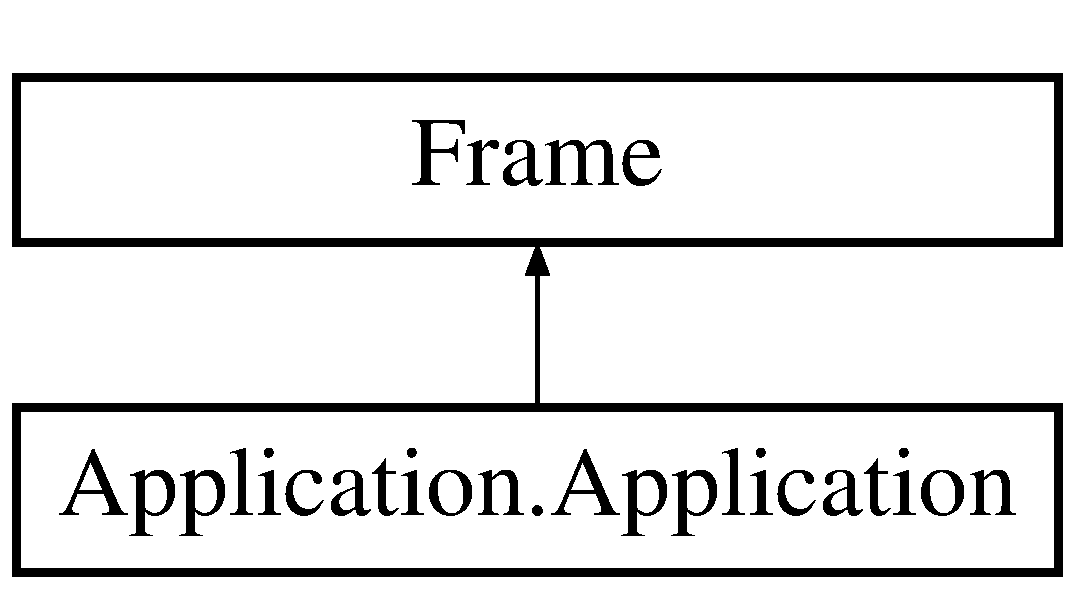
\includegraphics[height=2.000000cm]{class_application_1_1_application}
\end{center}
\end{figure}
\subsection*{Public Member Functions}
\begin{DoxyCompactItemize}
\item 
def \textbf{ key} (self, event)
\item 
def \textbf{ mouse\+\_\+press} (self, event)
\item 
def \textbf{ mouse\+\_\+release} (self, event)
\item 
def \textbf{ mouse\+\_\+motion} (self, event)
\item 
def \textbf{ Draw\+Point2D} (self, point, radius, color)
\item 
def \textbf{ Draw\+Colors2D} (self, R\+G\+BD, img)
\item 
def \textbf{ Draw\+Skeleton2D} (self, Pose)
\item 
def \textbf{ Draw\+Centers2D} (self, Pose, s=1)
\item 
def \textbf{ Draw\+Sys2D} (self, Pose)
\item 
def \textbf{ Draw\+O\+B\+Box2D} (self, Pose)
\item 
def \textbf{ \+\_\+\+\_\+init\+\_\+\+\_\+} (self, path, G\+P\+U\+Manager, master=None)
\begin{DoxyCompactList}\small\item\em Constructor function. \end{DoxyCompactList}\end{DoxyCompactItemize}
\subsection*{Public Attributes}
\begin{DoxyCompactItemize}
\item 
\mbox{\label{class_application_1_1_application_a643b31e93e0bc05341e57ba468b4f6f3}} 
{\bfseries color\+\_\+tag}
\item 
\mbox{\label{class_application_1_1_application_ada6d6879848e900c1850c9392c4f470e}} 
{\bfseries Pose}
\item 
\mbox{\label{class_application_1_1_application_aca0834aa1c44002fe610ebc80dec0ecc}} 
{\bfseries img\+Tk}
\item 
\mbox{\label{class_application_1_1_application_a73a85463ff9f37fdf7b37c6a8ddfc6b9}} 
{\bfseries x\+\_\+init}
\item 
\mbox{\label{class_application_1_1_application_a29a38708c2931c1bf01e083580d6cb65}} 
{\bfseries y\+\_\+init}
\item 
\mbox{\label{class_application_1_1_application_a224f9ee994b50b04544ef4a672e63ed4}} 
{\bfseries ctr2D}
\item 
\mbox{\label{class_application_1_1_application_a51bf1a1fd9739a8b1ac39ee6cab97f56}} 
{\bfseries O\+B\+Bcoords2D}
\item 
\mbox{\label{class_application_1_1_application_af0ed58988ec61974ed3df13e0efadd48}} 
{\bfseries root}
\item 
\mbox{\label{class_application_1_1_application_afdc18a45655b60e479c8e8abdff0d817}} 
{\bfseries path}
\item 
\mbox{\label{class_application_1_1_application_a642089891b00ec772170b0cc4b71431d}} 
{\bfseries G\+P\+U\+Manager}
\item 
\mbox{\label{class_application_1_1_application_ac0a98c12024e47d785358ef75fded13a}} 
{\bfseries draw\+\_\+bump}
\item 
\mbox{\label{class_application_1_1_application_aa89a81a42a52f24b4c9816cabd80e303}} 
{\bfseries draw\+\_\+spline}
\item 
\mbox{\label{class_application_1_1_application_a6b35840e9d7dda2ffb68b21f05f69825}} 
{\bfseries Size}
\item 
\mbox{\label{class_application_1_1_application_ad9df94fccad5a2ab7c7289fd03e11cc8}} 
{\bfseries intrinsic}
\item 
\mbox{\label{class_application_1_1_application_a5621b526d04bbb3e01c79aa2de0f6f70}} 
{\bfseries pos2d}
\item 
\mbox{\label{class_application_1_1_application_a2f8ef7d7d559d8a1fc7cdb4ab7dfedb7}} 
{\bfseries connection\+Mat}
\item 
\mbox{\label{class_application_1_1_application_a7b6a9840a20831ee3603358f862d8dac}} 
{\bfseries connection}
\item 
\mbox{\label{class_application_1_1_application_a3e83156042a91a7ac51b43a212af1b15}} 
{\bfseries Index}
\item 
\mbox{\label{class_application_1_1_application_af014bd8cb86e29f59612d916bf086776}} 
{\bfseries R\+G\+BD}
\item 
\mbox{\label{class_application_1_1_application_ad24990f1b38142dd639d7bd895638de7}} 
{\bfseries canvas}
\item 
\mbox{\label{class_application_1_1_application_a252c7894fa91a112d1238a760346d6b9}} 
{\bfseries w}
\end{DoxyCompactItemize}


\subsection{Detailed Description}
\begin{DoxyVerb}Class to apply the segmented fusion
It also contains function to handle keyboard and mouse inputs
\end{DoxyVerb}
 

\subsection{Constructor \& Destructor Documentation}
\mbox{\label{class_application_1_1_application_a0a1efa05f27e797bfc72d43dd12df6b5}} 
\index{Application\+::\+Application@{Application\+::\+Application}!\+\_\+\+\_\+init\+\_\+\+\_\+@{\+\_\+\+\_\+init\+\_\+\+\_\+}}
\index{\+\_\+\+\_\+init\+\_\+\+\_\+@{\+\_\+\+\_\+init\+\_\+\+\_\+}!Application\+::\+Application@{Application\+::\+Application}}
\subsubsection{\+\_\+\+\_\+init\+\_\+\+\_\+()}
{\footnotesize\ttfamily def Application.\+Application.\+\_\+\+\_\+init\+\_\+\+\_\+ (\begin{DoxyParamCaption}\item[{}]{self,  }\item[{}]{path,  }\item[{}]{G\+P\+U\+Manager,  }\item[{}]{master = {\ttfamily None} }\end{DoxyParamCaption})}



Constructor function. 

\begin{DoxyVerb}Main function of the project
:param path: path to search data
:param GPUManager: GPU environment
:param master: none
\end{DoxyVerb}
 

\subsection{Member Function Documentation}
\mbox{\label{class_application_1_1_application_a3280e6b8e4616a56567d0daf7f60ff23}} 
\index{Application\+::\+Application@{Application\+::\+Application}!Draw\+Centers2D@{Draw\+Centers2D}}
\index{Draw\+Centers2D@{Draw\+Centers2D}!Application\+::\+Application@{Application\+::\+Application}}
\subsubsection{Draw\+Centers2\+D()}
{\footnotesize\ttfamily def Application.\+Application.\+Draw\+Centers2D (\begin{DoxyParamCaption}\item[{}]{self,  }\item[{}]{Pose,  }\item[{}]{s = {\ttfamily 1} }\end{DoxyParamCaption})}

\begin{DoxyVerb}this function draw the center of each oriented coordinates system for each body part\end{DoxyVerb}
 \mbox{\label{class_application_1_1_application_a935ca95709286fee970c85727bf5bab4}} 
\index{Application\+::\+Application@{Application\+::\+Application}!Draw\+Colors2D@{Draw\+Colors2D}}
\index{Draw\+Colors2D@{Draw\+Colors2D}!Application\+::\+Application@{Application\+::\+Application}}
\subsubsection{Draw\+Colors2\+D()}
{\footnotesize\ttfamily def Application.\+Application.\+Draw\+Colors2D (\begin{DoxyParamCaption}\item[{}]{self,  }\item[{}]{R\+G\+BD,  }\item[{}]{img }\end{DoxyParamCaption})}

\begin{DoxyVerb}Draw the color of each segmented part of the body
:param RGBD:
:param img:
:param Pose:
:return:
Adding an argument pose would enable to follow the transformation
\end{DoxyVerb}
 \mbox{\label{class_application_1_1_application_a766ac4121a3cd61ad34b957bced90427}} 
\index{Application\+::\+Application@{Application\+::\+Application}!Draw\+O\+B\+Box2D@{Draw\+O\+B\+Box2D}}
\index{Draw\+O\+B\+Box2D@{Draw\+O\+B\+Box2D}!Application\+::\+Application@{Application\+::\+Application}}
\subsubsection{Draw\+O\+B\+Box2\+D()}
{\footnotesize\ttfamily def Application.\+Application.\+Draw\+O\+B\+Box2D (\begin{DoxyParamCaption}\item[{}]{self,  }\item[{}]{Pose }\end{DoxyParamCaption})}

\begin{DoxyVerb}Draw in the canvas the Oriented Bounding Boxes (OBB) for each body part
\end{DoxyVerb}
 \mbox{\label{class_application_1_1_application_a6564aeb78321ccf643be0b90fe2b388e}} 
\index{Application\+::\+Application@{Application\+::\+Application}!Draw\+Point2D@{Draw\+Point2D}}
\index{Draw\+Point2D@{Draw\+Point2D}!Application\+::\+Application@{Application\+::\+Application}}
\subsubsection{Draw\+Point2\+D()}
{\footnotesize\ttfamily def Application.\+Application.\+Draw\+Point2D (\begin{DoxyParamCaption}\item[{}]{self,  }\item[{}]{point,  }\item[{}]{radius,  }\item[{}]{color }\end{DoxyParamCaption})}

\begin{DoxyVerb}Draw a point in the image
:param point: 2D coordinates
:param radius: size of the point
:param color: Color of the point
:return: none
\end{DoxyVerb}
 \mbox{\label{class_application_1_1_application_af36ed2ae19b0450de779306b410dee6f}} 
\index{Application\+::\+Application@{Application\+::\+Application}!Draw\+Skeleton2D@{Draw\+Skeleton2D}}
\index{Draw\+Skeleton2D@{Draw\+Skeleton2D}!Application\+::\+Application@{Application\+::\+Application}}
\subsubsection{Draw\+Skeleton2\+D()}
{\footnotesize\ttfamily def Application.\+Application.\+Draw\+Skeleton2D (\begin{DoxyParamCaption}\item[{}]{self,  }\item[{}]{Pose }\end{DoxyParamCaption})}

\begin{DoxyVerb}Sraw the Skeleton of a human and make connections between each part
:param Pose:
:return:
Adding an argument pose would enable to follow the transformation
\end{DoxyVerb}
 \mbox{\label{class_application_1_1_application_a24fadbdd7cf0f4318724996b626e8c66}} 
\index{Application\+::\+Application@{Application\+::\+Application}!Draw\+Sys2D@{Draw\+Sys2D}}
\index{Draw\+Sys2D@{Draw\+Sys2D}!Application\+::\+Application@{Application\+::\+Application}}
\subsubsection{Draw\+Sys2\+D()}
{\footnotesize\ttfamily def Application.\+Application.\+Draw\+Sys2D (\begin{DoxyParamCaption}\item[{}]{self,  }\item[{}]{Pose }\end{DoxyParamCaption})}

\begin{DoxyVerb}this function draw the sys of oriented coordinates system for each body part\end{DoxyVerb}
 \mbox{\label{class_application_1_1_application_a7f10b75f569cab5769291c54ca1d3762}} 
\index{Application\+::\+Application@{Application\+::\+Application}!key@{key}}
\index{key@{key}!Application\+::\+Application@{Application\+::\+Application}}
\subsubsection{key()}
{\footnotesize\ttfamily def Application.\+Application.\+key (\begin{DoxyParamCaption}\item[{}]{self,  }\item[{}]{event }\end{DoxyParamCaption})}

\begin{DoxyVerb}Function to handle keyboard inputs
:param event: press a button on the keyboard
:return: none
\end{DoxyVerb}
 \mbox{\label{class_application_1_1_application_a1a6c84b431acbb546e466eaab2141e51}} 
\index{Application\+::\+Application@{Application\+::\+Application}!mouse\+\_\+motion@{mouse\+\_\+motion}}
\index{mouse\+\_\+motion@{mouse\+\_\+motion}!Application\+::\+Application@{Application\+::\+Application}}
\subsubsection{mouse\+\_\+motion()}
{\footnotesize\ttfamily def Application.\+Application.\+mouse\+\_\+motion (\begin{DoxyParamCaption}\item[{}]{self,  }\item[{}]{event }\end{DoxyParamCaption})}

\begin{DoxyVerb}Function to handle mouse motion events. displacement related to the event
:param event: moving mouse when a button is pressed
:return: none
\end{DoxyVerb}
 \mbox{\label{class_application_1_1_application_ab71deae47ac8b52b81ca833c5fdd3da0}} 
\index{Application\+::\+Application@{Application\+::\+Application}!mouse\+\_\+press@{mouse\+\_\+press}}
\index{mouse\+\_\+press@{mouse\+\_\+press}!Application\+::\+Application@{Application\+::\+Application}}
\subsubsection{mouse\+\_\+press()}
{\footnotesize\ttfamily def Application.\+Application.\+mouse\+\_\+press (\begin{DoxyParamCaption}\item[{}]{self,  }\item[{}]{event }\end{DoxyParamCaption})}

\begin{DoxyVerb}Function to handle mouse press event, displacement related to the event
:param event: a click with the mouse
:return: none\end{DoxyVerb}
 \mbox{\label{class_application_1_1_application_a239b47672cfb2b3e71302d0536a54e82}} 
\index{Application\+::\+Application@{Application\+::\+Application}!mouse\+\_\+release@{mouse\+\_\+release}}
\index{mouse\+\_\+release@{mouse\+\_\+release}!Application\+::\+Application@{Application\+::\+Application}}
\subsubsection{mouse\+\_\+release()}
{\footnotesize\ttfamily def Application.\+Application.\+mouse\+\_\+release (\begin{DoxyParamCaption}\item[{}]{self,  }\item[{}]{event }\end{DoxyParamCaption})}

\begin{DoxyVerb}Function to handle mouse release events, displacement related to the event
:param event: a click with the mouse
:return: none
\end{DoxyVerb}
 

The documentation for this class was generated from the following file\+:\begin{DoxyCompactItemize}
\item 
lib/Application.\+py\end{DoxyCompactItemize}

\hypertarget{class_body_parts_1_1_body_parts}{}\section{Body\+Parts.\+Body\+Parts Class Reference}
\label{class_body_parts_1_1_body_parts}\index{Body\+Parts.\+Body\+Parts@{Body\+Parts.\+Body\+Parts}}
\subsection*{Public Member Functions}
\begin{DoxyCompactItemize}
\item 
def \hyperlink{class_body_parts_1_1_body_parts_a1d480c13f6791c93e0da18d6da99a785}{\+\_\+\+\_\+init\+\_\+\+\_\+} (self, G\+P\+U\+Manager, R\+G\+BD, R\+G\+B\+D\+\_\+\+BP, Tlg)
\item 
def \hyperlink{class_body_parts_1_1_body_parts_a42e88badcb71b203213ef853ff7aa291}{Model3\+D\+\_\+init} (self, bp)
\end{DoxyCompactItemize}
\subsection*{Public Attributes}
\begin{DoxyCompactItemize}
\item 
\mbox{\Hypertarget{class_body_parts_1_1_body_parts_ab3a2fc59ff473104c3f51a2f3f9c5010}\label{class_body_parts_1_1_body_parts_ab3a2fc59ff473104c3f51a2f3f9c5010}} 
{\bfseries G\+P\+U\+Manager}
\item 
\mbox{\Hypertarget{class_body_parts_1_1_body_parts_ac1812d58953dcb8afbc9e1f3265e7ca4}\label{class_body_parts_1_1_body_parts_ac1812d58953dcb8afbc9e1f3265e7ca4}} 
{\bfseries R\+G\+BD}
\item 
\mbox{\Hypertarget{class_body_parts_1_1_body_parts_a39bad48cedf4b87ed875975ff13bd642}\label{class_body_parts_1_1_body_parts_a39bad48cedf4b87ed875975ff13bd642}} 
{\bfseries Tlg}
\item 
\mbox{\Hypertarget{class_body_parts_1_1_body_parts_a7f470c49a980e43e653f020e62ab7365}\label{class_body_parts_1_1_body_parts_a7f470c49a980e43e653f020e62ab7365}} 
{\bfseries R\+G\+B\+D\+\_\+\+BP}
\item 
\mbox{\Hypertarget{class_body_parts_1_1_body_parts_ab1441a0be27dc35510f8ab0d450a5059}\label{class_body_parts_1_1_body_parts_ab1441a0be27dc35510f8ab0d450a5059}} 
{\bfseries Vox\+Size}
\item 
\mbox{\Hypertarget{class_body_parts_1_1_body_parts_afbbad8811acdf0e0ecaf8f2a62b5e00d}\label{class_body_parts_1_1_body_parts_afbbad8811acdf0e0ecaf8f2a62b5e00d}} 
{\bfseries T\+S\+D\+F\+Manager}
\item 
\mbox{\Hypertarget{class_body_parts_1_1_body_parts_a461ad5d0d38ec1e94a0162f4f560f3c3}\label{class_body_parts_1_1_body_parts_a461ad5d0d38ec1e94a0162f4f560f3c3}} 
{\bfseries MC}
\end{DoxyCompactItemize}


\subsection{Detailed Description}
\begin{DoxyVerb}Body parts
\end{DoxyVerb}
 

\subsection{Constructor \& Destructor Documentation}
\mbox{\Hypertarget{class_body_parts_1_1_body_parts_a1d480c13f6791c93e0da18d6da99a785}\label{class_body_parts_1_1_body_parts_a1d480c13f6791c93e0da18d6da99a785}} 
\index{Body\+Parts\+::\+Body\+Parts@{Body\+Parts\+::\+Body\+Parts}!\+\_\+\+\_\+init\+\_\+\+\_\+@{\+\_\+\+\_\+init\+\_\+\+\_\+}}
\index{\+\_\+\+\_\+init\+\_\+\+\_\+@{\+\_\+\+\_\+init\+\_\+\+\_\+}!Body\+Parts\+::\+Body\+Parts@{Body\+Parts\+::\+Body\+Parts}}
\subsubsection{\texorpdfstring{\+\_\+\+\_\+init\+\_\+\+\_\+()}{\_\_init\_\_()}}
{\footnotesize\ttfamily def Body\+Parts.\+Body\+Parts.\+\_\+\+\_\+init\+\_\+\+\_\+ (\begin{DoxyParamCaption}\item[{}]{self,  }\item[{}]{G\+P\+U\+Manager,  }\item[{}]{R\+G\+BD,  }\item[{}]{R\+G\+B\+D\+\_\+\+BP,  }\item[{}]{Tlg }\end{DoxyParamCaption})}

\begin{DoxyVerb}Init a body parts
:param GPUManager: GPU environment
:param RGBD: Image having all the body
:param RGBD_BP: Image containing just the body part
:param Tlg: Transform local to global for the concerned body parts
\end{DoxyVerb}
 

\subsection{Member Function Documentation}
\mbox{\Hypertarget{class_body_parts_1_1_body_parts_a42e88badcb71b203213ef853ff7aa291}\label{class_body_parts_1_1_body_parts_a42e88badcb71b203213ef853ff7aa291}} 
\index{Body\+Parts\+::\+Body\+Parts@{Body\+Parts\+::\+Body\+Parts}!Model3\+D\+\_\+init@{Model3\+D\+\_\+init}}
\index{Model3\+D\+\_\+init@{Model3\+D\+\_\+init}!Body\+Parts\+::\+Body\+Parts@{Body\+Parts\+::\+Body\+Parts}}
\subsubsection{\texorpdfstring{Model3\+D\+\_\+init()}{Model3D\_init()}}
{\footnotesize\ttfamily def Body\+Parts.\+Body\+Parts.\+Model3\+D\+\_\+init (\begin{DoxyParamCaption}\item[{}]{self,  }\item[{}]{bp }\end{DoxyParamCaption})}

\begin{DoxyVerb}Create a 3D model of the body parts
:param bp: number of the body part
:return:  none
\end{DoxyVerb}
 

The documentation for this class was generated from the following file\+:\begin{DoxyCompactItemize}
\item 
code/lib/Body\+Parts.\+py\end{DoxyCompactItemize}

\section{G\+P\+U\+Manager.\+G\+P\+U\+Manager Class Reference}
\label{class_g_p_u_manager_1_1_g_p_u_manager}\index{G\+P\+U\+Manager.\+G\+P\+U\+Manager@{G\+P\+U\+Manager.\+G\+P\+U\+Manager}}
\subsection*{Public Member Functions}
\begin{DoxyCompactItemize}
\item 
def \textbf{ \+\_\+\+\_\+init\+\_\+\+\_\+} (self)
\item 
def \textbf{ print\+\_\+device\+\_\+info} (self)
\item 
def \textbf{ load\+\_\+kernels} (self)
\end{DoxyCompactItemize}
\subsection*{Public Attributes}
\begin{DoxyCompactItemize}
\item 
\mbox{\label{class_g_p_u_manager_1_1_g_p_u_manager_ae95df47a91b17aa5a9f045efd0547416}} 
{\bfseries platform}
\item 
\mbox{\label{class_g_p_u_manager_1_1_g_p_u_manager_aec4090621f66cd5d003c6c4d6a40ccaa}} 
{\bfseries devices}
\item 
\mbox{\label{class_g_p_u_manager_1_1_g_p_u_manager_a6c40884972be2350ea61b03a11339354}} 
{\bfseries context}
\item 
\mbox{\label{class_g_p_u_manager_1_1_g_p_u_manager_ad4d3c25e7aa7a1ecf7683d6c3a4a3350}} 
{\bfseries queue}
\item 
\mbox{\label{class_g_p_u_manager_1_1_g_p_u_manager_ae25153bc81d73a1744fa80d8c994ee06}} 
{\bfseries programs}
\end{DoxyCompactItemize}


\subsection{Detailed Description}
\begin{DoxyVerb}GPUManager is the class that initialized GPU envirenment and functions

Work-item: the basic unit of work on an OpenCL device
Kernel: the code for a work-item (basically a C function)
Program: Collection of kernels and other functions (analogous to a dynamic library)
Context: The environment within which workitems execute; includes devices and their memories and command queues
Command Queue: A queue used by the Host application to submit work to a Device (e.g., kernel execution instances)
                Namely, it is control work order.
   – Work is queued in-order, one queue per device
   – Work can be executed in-order or out-of-order
Platform: The host plus a collection of devices managed by the OpenCL framework that allow an application to share resources and execute kernels on devices in the platform.
\end{DoxyVerb}
 

\subsection{Constructor \& Destructor Documentation}
\mbox{\label{class_g_p_u_manager_1_1_g_p_u_manager_aaa00d0d2f90d9cb6bab88f873d3e1261}} 
\index{G\+P\+U\+Manager\+::\+G\+P\+U\+Manager@{G\+P\+U\+Manager\+::\+G\+P\+U\+Manager}!\+\_\+\+\_\+init\+\_\+\+\_\+@{\+\_\+\+\_\+init\+\_\+\+\_\+}}
\index{\+\_\+\+\_\+init\+\_\+\+\_\+@{\+\_\+\+\_\+init\+\_\+\+\_\+}!G\+P\+U\+Manager\+::\+G\+P\+U\+Manager@{G\+P\+U\+Manager\+::\+G\+P\+U\+Manager}}
\subsubsection{\+\_\+\+\_\+init\+\_\+\+\_\+()}
{\footnotesize\ttfamily def G\+P\+U\+Manager.\+G\+P\+U\+Manager.\+\_\+\+\_\+init\+\_\+\+\_\+ (\begin{DoxyParamCaption}\item[{}]{self }\end{DoxyParamCaption})}

\begin{DoxyVerb}Constructor
\end{DoxyVerb}
 

\subsection{Member Function Documentation}
\mbox{\label{class_g_p_u_manager_1_1_g_p_u_manager_a95ccd16d4a81b00946d87f91bdca27e9}} 
\index{G\+P\+U\+Manager\+::\+G\+P\+U\+Manager@{G\+P\+U\+Manager\+::\+G\+P\+U\+Manager}!load\+\_\+kernels@{load\+\_\+kernels}}
\index{load\+\_\+kernels@{load\+\_\+kernels}!G\+P\+U\+Manager\+::\+G\+P\+U\+Manager@{G\+P\+U\+Manager\+::\+G\+P\+U\+Manager}}
\subsubsection{load\+\_\+kernels()}
{\footnotesize\ttfamily def G\+P\+U\+Manager.\+G\+P\+U\+Manager.\+load\+\_\+kernels (\begin{DoxyParamCaption}\item[{}]{self }\end{DoxyParamCaption})}

\begin{DoxyVerb}Load programs with its kernels
:return: none
\end{DoxyVerb}
 \mbox{\label{class_g_p_u_manager_1_1_g_p_u_manager_a936c21f2d21ae94b581636e9255e71df}} 
\index{G\+P\+U\+Manager\+::\+G\+P\+U\+Manager@{G\+P\+U\+Manager\+::\+G\+P\+U\+Manager}!print\+\_\+device\+\_\+info@{print\+\_\+device\+\_\+info}}
\index{print\+\_\+device\+\_\+info@{print\+\_\+device\+\_\+info}!G\+P\+U\+Manager\+::\+G\+P\+U\+Manager@{G\+P\+U\+Manager\+::\+G\+P\+U\+Manager}}
\subsubsection{print\+\_\+device\+\_\+info()}
{\footnotesize\ttfamily def G\+P\+U\+Manager.\+G\+P\+U\+Manager.\+print\+\_\+device\+\_\+info (\begin{DoxyParamCaption}\item[{}]{self }\end{DoxyParamCaption})}

\begin{DoxyVerb}Display information on selected devices
:return:  none
\end{DoxyVerb}
 

The documentation for this class was generated from the following file\+:\begin{DoxyCompactItemize}
\item 
lib/G\+P\+U\+Manager.\+py\end{DoxyCompactItemize}

\hypertarget{class_menu_1_1_menu}{}\section{Menu.\+Menu Class Reference}
\label{class_menu_1_1_menu}\index{Menu.\+Menu@{Menu.\+Menu}}
Inheritance diagram for Menu.\+Menu\+:\begin{figure}[H]
\begin{center}
\leavevmode
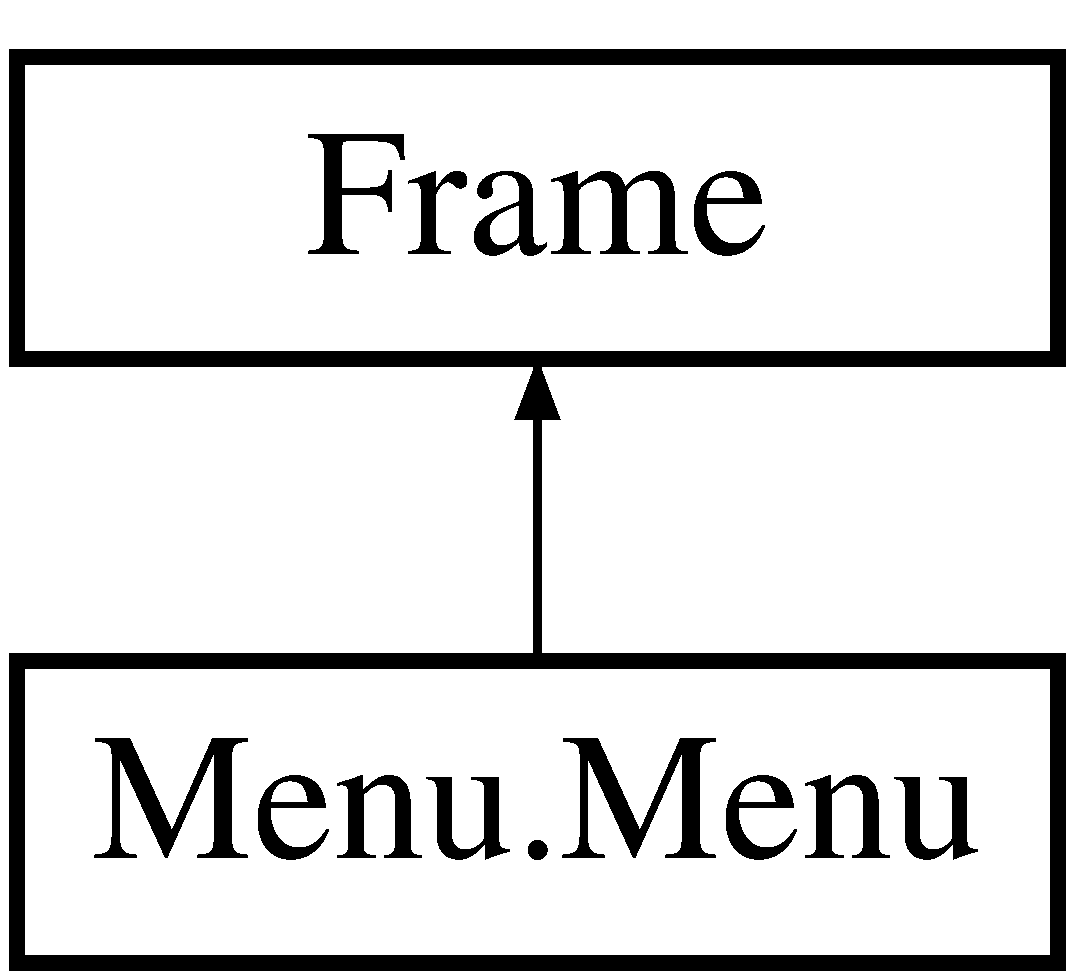
\includegraphics[height=2.000000cm]{class_menu_1_1_menu}
\end{center}
\end{figure}
\subsection*{Public Member Functions}
\begin{DoxyCompactItemize}
\item 
\mbox{\Hypertarget{class_menu_1_1_menu_a192785b95591dc7bdc5faf0d2bb56d27}\label{class_menu_1_1_menu_a192785b95591dc7bdc5faf0d2bb56d27}} 
def {\bfseries key} (self, event)
\item 
\mbox{\Hypertarget{class_menu_1_1_menu_a6dd74d36fda2d88998fba863f029bfe1}\label{class_menu_1_1_menu_a6dd74d36fda2d88998fba863f029bfe1}} 
def {\bfseries callback} (self, event)
\item 
\mbox{\Hypertarget{class_menu_1_1_menu_a06cf9e4a3865a0fdbf5a04ea44b6c13b}\label{class_menu_1_1_menu_a06cf9e4a3865a0fdbf5a04ea44b6c13b}} 
def {\bfseries \+\_\+\+\_\+init\+\_\+\+\_\+} (self, master=None)
\end{DoxyCompactItemize}
\subsection*{Public Attributes}
\begin{DoxyCompactItemize}
\item 
\mbox{\Hypertarget{class_menu_1_1_menu_a1e517ddc55633da361d27e455422ffbc}\label{class_menu_1_1_menu_a1e517ddc55633da361d27e455422ffbc}} 
{\bfseries filename}
\item 
\mbox{\Hypertarget{class_menu_1_1_menu_a4cd78a3815634c8b6702d188c8c0f538}\label{class_menu_1_1_menu_a4cd78a3815634c8b6702d188c8c0f538}} 
{\bfseries root}
\item 
\mbox{\Hypertarget{class_menu_1_1_menu_abc5dc4ee892cf12184228f2e138a3d6b}\label{class_menu_1_1_menu_abc5dc4ee892cf12184228f2e138a3d6b}} 
{\bfseries canvas}
\item 
\mbox{\Hypertarget{class_menu_1_1_menu_abaaf9d372dbc077c24ba14d061bc01f1}\label{class_menu_1_1_menu_abaaf9d372dbc077c24ba14d061bc01f1}} 
{\bfseries menu}
\item 
\mbox{\Hypertarget{class_menu_1_1_menu_a7e768c5029f17d0fa48bbdac18f524d2}\label{class_menu_1_1_menu_a7e768c5029f17d0fa48bbdac18f524d2}} 
{\bfseries menu\+\_\+label}
\end{DoxyCompactItemize}


\subsection{Detailed Description}
\begin{DoxyVerb}Class to handle menu GUI
\end{DoxyVerb}
 

The documentation for this class was generated from the following file\+:\begin{DoxyCompactItemize}
\item 
code/lib/Menu.\+py\end{DoxyCompactItemize}

\section{My\+\_\+\+Marching\+Cube.\+My\+\_\+\+Marching\+Cube Class Reference}
\label{class_my___marching_cube_1_1_my___marching_cube}\index{My\+\_\+\+Marching\+Cube.\+My\+\_\+\+Marching\+Cube@{My\+\_\+\+Marching\+Cube.\+My\+\_\+\+Marching\+Cube}}
\subsection*{Public Member Functions}
\begin{DoxyCompactItemize}
\item 
def \textbf{ \+\_\+\+\_\+init\+\_\+\+\_\+} (self, Size, Res, Iso, G\+P\+U\+Manager)
\item 
def \textbf{ run\+G\+PU} (self, Vol\+G\+PU)
\item 
def \textbf{ Save\+To\+Ply} (self, name, display=0)
\item 
def \textbf{ Save\+To\+Ply\+Ext} (self, name, nb\+\_\+vertices, nb\+\_\+faces, Vertices, Faces, display=0)
\item 
def \textbf{ Draw\+Mesh} (self, Pose, intrinsic, Size, canvas)
\item 
def \textbf{ Draw\+Points} (self, Pose, intrinsic, Size, background, s=1)
\item 
def \textbf{ Transform\+List} (self, Pose)
\item 
def \textbf{ Compute\+M\+C\+Nmls} (self)
\item 
def \textbf{ Compute\+M\+C\+Nmls\+\_\+slow} (self)
\item 
def \textbf{ Merge\+Vtx} (self)
\item 
def \textbf{ M\+C2\+R\+G\+BD} (self, R\+G\+BD, Vtx, Nmls, Pose, s, color=0)
\end{DoxyCompactItemize}
\subsection*{Public Attributes}
\begin{DoxyCompactItemize}
\item 
\mbox{\label{class_my___marching_cube_1_1_my___marching_cube_afe2f5faf0ce2a333474f9d1496192f14}} 
{\bfseries Size}
\item 
\mbox{\label{class_my___marching_cube_1_1_my___marching_cube_a4ecd41f50f60bf712ad456a8fc941782}} 
{\bfseries res}
\item 
\mbox{\label{class_my___marching_cube_1_1_my___marching_cube_a3dcab76028b44472b20e598b7532a217}} 
{\bfseries iso}
\item 
\mbox{\label{class_my___marching_cube_1_1_my___marching_cube_a8a75f5324dfcfbd3fab050edd4006998}} 
{\bfseries nb\+\_\+faces}
\item 
\mbox{\label{class_my___marching_cube_1_1_my___marching_cube_a908d5321153e2341f710c047d95ad01a}} 
{\bfseries G\+P\+U\+Manager}
\item 
\mbox{\label{class_my___marching_cube_1_1_my___marching_cube_a328ca204253663c7dc82f6497796c63a}} 
{\bfseries Size\+\_\+\+Volume}
\item 
\mbox{\label{class_my___marching_cube_1_1_my___marching_cube_a896f6c74b604e6b2135845e8d17d3977}} 
{\bfseries Offset\+G\+PU}
\item 
\mbox{\label{class_my___marching_cube_1_1_my___marching_cube_a0fe61051ce01b62f304ae085ac9bfb3a}} 
{\bfseries Index\+G\+PU}
\item 
\mbox{\label{class_my___marching_cube_1_1_my___marching_cube_ab77b74495b2578c0a35c8ca3d3876de9}} 
{\bfseries Face\+Counter\+G\+PU}
\item 
\mbox{\label{class_my___marching_cube_1_1_my___marching_cube_a52820bb2f10966fb592ec7d62c108d54}} 
{\bfseries Param\+G\+PU}
\item 
\mbox{\label{class_my___marching_cube_1_1_my___marching_cube_aceb2a4ed570e10e042a44a29cad5ea95}} 
{\bfseries Faces}
\item 
\mbox{\label{class_my___marching_cube_1_1_my___marching_cube_a800426654b2cf0feb64d1bf212b34921}} 
{\bfseries Vertices}
\item 
\mbox{\label{class_my___marching_cube_1_1_my___marching_cube_afa52802741219118770c709e75446d5e}} 
{\bfseries Faces\+G\+PU}
\item 
\mbox{\label{class_my___marching_cube_1_1_my___marching_cube_ac3124bef4e245b03d3e66982aab263c9}} 
{\bfseries Vertices\+G\+PU}
\item 
\mbox{\label{class_my___marching_cube_1_1_my___marching_cube_a9699fa7abe4cae11215828c4e55e2805}} 
{\bfseries Normales}
\item 
\mbox{\label{class_my___marching_cube_1_1_my___marching_cube_a6470869842e5e29387ce307bde36c22c}} 
{\bfseries Normals}
\item 
\mbox{\label{class_my___marching_cube_1_1_my___marching_cube_a03cbb9a458d30723be59caaecbc5310b}} 
{\bfseries nb\+Vtx}
\item 
\mbox{\label{class_my___marching_cube_1_1_my___marching_cube_a81808a234dcc9b8a1d0f7fe737b747ec}} 
{\bfseries nb\+\_\+vertices}
\end{DoxyCompactItemize}


\subsection{Constructor \& Destructor Documentation}
\mbox{\label{class_my___marching_cube_1_1_my___marching_cube_a7f2970f295285729918604008fc7809f}} 
\index{My\+\_\+\+Marching\+Cube\+::\+My\+\_\+\+Marching\+Cube@{My\+\_\+\+Marching\+Cube\+::\+My\+\_\+\+Marching\+Cube}!\+\_\+\+\_\+init\+\_\+\+\_\+@{\+\_\+\+\_\+init\+\_\+\+\_\+}}
\index{\+\_\+\+\_\+init\+\_\+\+\_\+@{\+\_\+\+\_\+init\+\_\+\+\_\+}!My\+\_\+\+Marching\+Cube\+::\+My\+\_\+\+Marching\+Cube@{My\+\_\+\+Marching\+Cube\+::\+My\+\_\+\+Marching\+Cube}}
\subsubsection{\+\_\+\+\_\+init\+\_\+\+\_\+()}
{\footnotesize\ttfamily def My\+\_\+\+Marching\+Cube.\+My\+\_\+\+Marching\+Cube.\+\_\+\+\_\+init\+\_\+\+\_\+ (\begin{DoxyParamCaption}\item[{}]{self,  }\item[{}]{Size,  }\item[{}]{Res,  }\item[{}]{Iso,  }\item[{}]{G\+P\+U\+Manager }\end{DoxyParamCaption})}

\begin{DoxyVerb}Constructor
:param Size: Size of the volume
:param Res: resolution parameters
:param Iso: isosurface to render
:param GPUManager: GPU environment
\end{DoxyVerb}
 

\subsection{Member Function Documentation}
\mbox{\label{class_my___marching_cube_1_1_my___marching_cube_a5a1e9c085022497596ba726002435603}} 
\index{My\+\_\+\+Marching\+Cube\+::\+My\+\_\+\+Marching\+Cube@{My\+\_\+\+Marching\+Cube\+::\+My\+\_\+\+Marching\+Cube}!Compute\+M\+C\+Nmls@{Compute\+M\+C\+Nmls}}
\index{Compute\+M\+C\+Nmls@{Compute\+M\+C\+Nmls}!My\+\_\+\+Marching\+Cube\+::\+My\+\_\+\+Marching\+Cube@{My\+\_\+\+Marching\+Cube\+::\+My\+\_\+\+Marching\+Cube}}
\subsubsection{Compute\+M\+C\+Nmls()}
{\footnotesize\ttfamily def My\+\_\+\+Marching\+Cube.\+My\+\_\+\+Marching\+Cube.\+Compute\+M\+C\+Nmls (\begin{DoxyParamCaption}\item[{}]{self }\end{DoxyParamCaption})}

\begin{DoxyVerb}    Function to compute the normals of the mesh
    NOT USED. (MergeVtx does the job)
\end{DoxyVerb}
 \mbox{\label{class_my___marching_cube_1_1_my___marching_cube_a27d160262d57b10e11ec11978c4fa8ea}} 
\index{My\+\_\+\+Marching\+Cube\+::\+My\+\_\+\+Marching\+Cube@{My\+\_\+\+Marching\+Cube\+::\+My\+\_\+\+Marching\+Cube}!Compute\+M\+C\+Nmls\+\_\+slow@{Compute\+M\+C\+Nmls\+\_\+slow}}
\index{Compute\+M\+C\+Nmls\+\_\+slow@{Compute\+M\+C\+Nmls\+\_\+slow}!My\+\_\+\+Marching\+Cube\+::\+My\+\_\+\+Marching\+Cube@{My\+\_\+\+Marching\+Cube\+::\+My\+\_\+\+Marching\+Cube}}
\subsubsection{Compute\+M\+C\+Nmls\+\_\+slow()}
{\footnotesize\ttfamily def My\+\_\+\+Marching\+Cube.\+My\+\_\+\+Marching\+Cube.\+Compute\+M\+C\+Nmls\+\_\+slow (\begin{DoxyParamCaption}\item[{}]{self }\end{DoxyParamCaption})}

\begin{DoxyVerb}Non optimized version for understanding
THIS FUNCTION IS NOT USED
\end{DoxyVerb}
 \mbox{\label{class_my___marching_cube_1_1_my___marching_cube_aa6b90ce7e02b9a41c824707630b64f07}} 
\index{My\+\_\+\+Marching\+Cube\+::\+My\+\_\+\+Marching\+Cube@{My\+\_\+\+Marching\+Cube\+::\+My\+\_\+\+Marching\+Cube}!Draw\+Mesh@{Draw\+Mesh}}
\index{Draw\+Mesh@{Draw\+Mesh}!My\+\_\+\+Marching\+Cube\+::\+My\+\_\+\+Marching\+Cube@{My\+\_\+\+Marching\+Cube\+::\+My\+\_\+\+Marching\+Cube}}
\subsubsection{Draw\+Mesh()}
{\footnotesize\ttfamily def My\+\_\+\+Marching\+Cube.\+My\+\_\+\+Marching\+Cube.\+Draw\+Mesh (\begin{DoxyParamCaption}\item[{}]{self,  }\item[{}]{Pose,  }\item[{}]{intrinsic,  }\item[{}]{Size,  }\item[{}]{canvas }\end{DoxyParamCaption})}

\begin{DoxyVerb}    Function to draw the mesh using tkinter
    NOT USED.
\end{DoxyVerb}
 \mbox{\label{class_my___marching_cube_1_1_my___marching_cube_a4b28f492fb09edfca2a4814c86631720}} 
\index{My\+\_\+\+Marching\+Cube\+::\+My\+\_\+\+Marching\+Cube@{My\+\_\+\+Marching\+Cube\+::\+My\+\_\+\+Marching\+Cube}!Draw\+Points@{Draw\+Points}}
\index{Draw\+Points@{Draw\+Points}!My\+\_\+\+Marching\+Cube\+::\+My\+\_\+\+Marching\+Cube@{My\+\_\+\+Marching\+Cube\+::\+My\+\_\+\+Marching\+Cube}}
\subsubsection{Draw\+Points()}
{\footnotesize\ttfamily def My\+\_\+\+Marching\+Cube.\+My\+\_\+\+Marching\+Cube.\+Draw\+Points (\begin{DoxyParamCaption}\item[{}]{self,  }\item[{}]{Pose,  }\item[{}]{intrinsic,  }\item[{}]{Size,  }\item[{}]{background,  }\item[{}]{s = {\ttfamily 1} }\end{DoxyParamCaption})}

\begin{DoxyVerb}    Function to draw the vertices of the mesh using tkinter
    NOT USED.
\end{DoxyVerb}
 \mbox{\label{class_my___marching_cube_1_1_my___marching_cube_aaf418aa2b8358d872fc53616408acdf6}} 
\index{My\+\_\+\+Marching\+Cube\+::\+My\+\_\+\+Marching\+Cube@{My\+\_\+\+Marching\+Cube\+::\+My\+\_\+\+Marching\+Cube}!M\+C2\+R\+G\+BD@{M\+C2\+R\+G\+BD}}
\index{M\+C2\+R\+G\+BD@{M\+C2\+R\+G\+BD}!My\+\_\+\+Marching\+Cube\+::\+My\+\_\+\+Marching\+Cube@{My\+\_\+\+Marching\+Cube\+::\+My\+\_\+\+Marching\+Cube}}
\subsubsection{M\+C2\+R\+G\+B\+D()}
{\footnotesize\ttfamily def My\+\_\+\+Marching\+Cube.\+My\+\_\+\+Marching\+Cube.\+M\+C2\+R\+G\+BD (\begin{DoxyParamCaption}\item[{}]{self,  }\item[{}]{R\+G\+BD,  }\item[{}]{Vtx,  }\item[{}]{Nmls,  }\item[{}]{Pose,  }\item[{}]{s,  }\item[{}]{color = {\ttfamily 0} }\end{DoxyParamCaption})}

\begin{DoxyVerb}    Function to convert the list of normales and vertexes of the marching cubes' algorithm into
    424*512*3 matrix.
    This function is made just to test with the RegisterRGBD function if the data from the mesh are corrects.
\end{DoxyVerb}
 \mbox{\label{class_my___marching_cube_1_1_my___marching_cube_a234beb0a06a023ee9d4571d569af755c}} 
\index{My\+\_\+\+Marching\+Cube\+::\+My\+\_\+\+Marching\+Cube@{My\+\_\+\+Marching\+Cube\+::\+My\+\_\+\+Marching\+Cube}!Merge\+Vtx@{Merge\+Vtx}}
\index{Merge\+Vtx@{Merge\+Vtx}!My\+\_\+\+Marching\+Cube\+::\+My\+\_\+\+Marching\+Cube@{My\+\_\+\+Marching\+Cube\+::\+My\+\_\+\+Marching\+Cube}}
\subsubsection{Merge\+Vtx()}
{\footnotesize\ttfamily def My\+\_\+\+Marching\+Cube.\+My\+\_\+\+Marching\+Cube.\+Merge\+Vtx (\begin{DoxyParamCaption}\item[{}]{self }\end{DoxyParamCaption})}

\begin{DoxyVerb}This function avoid having duplicate in the lists of vertexes or normales
THIS METHOD HAVE A GPU VERSION BUT THE GPU HAVE NOT ENOUGH MEMORY TO RUN IT
\end{DoxyVerb}
 \mbox{\label{class_my___marching_cube_1_1_my___marching_cube_a820edf1a7b295d5e3fbe858bddc03423}} 
\index{My\+\_\+\+Marching\+Cube\+::\+My\+\_\+\+Marching\+Cube@{My\+\_\+\+Marching\+Cube\+::\+My\+\_\+\+Marching\+Cube}!run\+G\+PU@{run\+G\+PU}}
\index{run\+G\+PU@{run\+G\+PU}!My\+\_\+\+Marching\+Cube\+::\+My\+\_\+\+Marching\+Cube@{My\+\_\+\+Marching\+Cube\+::\+My\+\_\+\+Marching\+Cube}}
\subsubsection{run\+G\+P\+U()}
{\footnotesize\ttfamily def My\+\_\+\+Marching\+Cube.\+My\+\_\+\+Marching\+Cube.\+run\+G\+PU (\begin{DoxyParamCaption}\item[{}]{self,  }\item[{}]{Vol\+G\+PU }\end{DoxyParamCaption})}

\begin{DoxyVerb}First find all the edges that are crossed by the surface
Second compute face and vertices according to the edges
Third merge duplicate (need to be optimize)
:param VolGPU: Volume given by the TSDF
:return: none
\end{DoxyVerb}
 \mbox{\label{class_my___marching_cube_1_1_my___marching_cube_a9ba8a5429eed6fbbe83798c4988e65f4}} 
\index{My\+\_\+\+Marching\+Cube\+::\+My\+\_\+\+Marching\+Cube@{My\+\_\+\+Marching\+Cube\+::\+My\+\_\+\+Marching\+Cube}!Save\+To\+Ply@{Save\+To\+Ply}}
\index{Save\+To\+Ply@{Save\+To\+Ply}!My\+\_\+\+Marching\+Cube\+::\+My\+\_\+\+Marching\+Cube@{My\+\_\+\+Marching\+Cube\+::\+My\+\_\+\+Marching\+Cube}}
\subsubsection{Save\+To\+Ply()}
{\footnotesize\ttfamily def My\+\_\+\+Marching\+Cube.\+My\+\_\+\+Marching\+Cube.\+Save\+To\+Ply (\begin{DoxyParamCaption}\item[{}]{self,  }\item[{}]{name,  }\item[{}]{display = {\ttfamily 0} }\end{DoxyParamCaption})}

\begin{DoxyVerb}Function to record the created mesh into a .ply file
Create file .ply with vertices and faces for vizualization in MeshLab
:param name: string, name of the file
:param times: 0 if you do not want to display the time
:return: none
\end{DoxyVerb}
 \mbox{\label{class_my___marching_cube_1_1_my___marching_cube_a9c250e7239f5e6a7f547ee18f0ad6e43}} 
\index{My\+\_\+\+Marching\+Cube\+::\+My\+\_\+\+Marching\+Cube@{My\+\_\+\+Marching\+Cube\+::\+My\+\_\+\+Marching\+Cube}!Save\+To\+Ply\+Ext@{Save\+To\+Ply\+Ext}}
\index{Save\+To\+Ply\+Ext@{Save\+To\+Ply\+Ext}!My\+\_\+\+Marching\+Cube\+::\+My\+\_\+\+Marching\+Cube@{My\+\_\+\+Marching\+Cube\+::\+My\+\_\+\+Marching\+Cube}}
\subsubsection{Save\+To\+Ply\+Ext()}
{\footnotesize\ttfamily def My\+\_\+\+Marching\+Cube.\+My\+\_\+\+Marching\+Cube.\+Save\+To\+Ply\+Ext (\begin{DoxyParamCaption}\item[{}]{self,  }\item[{}]{name,  }\item[{}]{nb\+\_\+vertices,  }\item[{}]{nb\+\_\+faces,  }\item[{}]{Vertices,  }\item[{}]{Faces,  }\item[{}]{display = {\ttfamily 0} }\end{DoxyParamCaption})}

\begin{DoxyVerb}Function to record an external created mesh into a .ply file
Create file .ply with vertices and faces for vizualization in MeshLab
:param name: string, name of the file
:param nb_vertices: int, number of vertices N*3
:param nb_faces: int, number of faces N
:param Vertices: array 3*N*3,
:param Faces: array N*3,
:param display: int, 0 if you do not want to display the time
:return: none
\end{DoxyVerb}
 \mbox{\label{class_my___marching_cube_1_1_my___marching_cube_a063b11ec768a65b5b73159c6eed61e32}} 
\index{My\+\_\+\+Marching\+Cube\+::\+My\+\_\+\+Marching\+Cube@{My\+\_\+\+Marching\+Cube\+::\+My\+\_\+\+Marching\+Cube}!Transform\+List@{Transform\+List}}
\index{Transform\+List@{Transform\+List}!My\+\_\+\+Marching\+Cube\+::\+My\+\_\+\+Marching\+Cube@{My\+\_\+\+Marching\+Cube\+::\+My\+\_\+\+Marching\+Cube}}
\subsubsection{Transform\+List()}
{\footnotesize\ttfamily def My\+\_\+\+Marching\+Cube.\+My\+\_\+\+Marching\+Cube.\+Transform\+List (\begin{DoxyParamCaption}\item[{}]{self,  }\item[{}]{Pose }\end{DoxyParamCaption})}

\begin{DoxyVerb}    Function to transform normals and vertices of the mesh
\end{DoxyVerb}
 

The documentation for this class was generated from the following file\+:\begin{DoxyCompactItemize}
\item 
lib/My\+\_\+\+Marching\+Cube.\+py\end{DoxyCompactItemize}

\hypertarget{class_r_g_b_d_1_1_r_g_b_d}{}\section{R\+G\+B\+D.\+R\+G\+BD Class Reference}
\label{class_r_g_b_d_1_1_r_g_b_d}\index{R\+G\+B\+D.\+R\+G\+BD@{R\+G\+B\+D.\+R\+G\+BD}}
\subsection*{Public Member Functions}
\begin{DoxyCompactItemize}
\item 
def \hyperlink{class_r_g_b_d_1_1_r_g_b_d_adf3e96f8b0620fd3f68b2399d29c3b12}{\+\_\+\+\_\+init\+\_\+\+\_\+} (self, depthname, colorname, intrinsic, fact)
\item 
def \hyperlink{class_r_g_b_d_1_1_r_g_b_d_accb9314bc9a43859adbcbb85283e3722}{Load\+Mat} (self, Images, Pos\+\_\+2D, Body\+Connection, bin\+Image)
\item 
def \hyperlink{class_r_g_b_d_1_1_r_g_b_d_a65ca0d3759c2b9977b24c952b9057ac9}{Read\+From\+Disk} (self)
\item 
def \hyperlink{class_r_g_b_d_1_1_r_g_b_d_ac7350dc76ae47fdd77c0ad93a74910db}{Read\+From\+Mat} (self, idx=-\/1)
\item 
def \hyperlink{class_r_g_b_d_1_1_r_g_b_d_a98624ce143f3ea4b766e337467faaf68}{Vmap} (self)
\begin{DoxyCompactList}\small\item\em Map Conversion Functions \#\#\#\#\#\#\#\#\#\#\#\#\#\#\#\#\#\#\#\#\#\#\#. \end{DoxyCompactList}\item 
def \hyperlink{class_r_g_b_d_1_1_r_g_b_d_a2686c0b37c9c4cf8a650656680402797}{Vmap\+\_\+optimize} (self)
\item 
def \hyperlink{class_r_g_b_d_1_1_r_g_b_d_a9cba8018f1cdb3f5c73c863a49549061}{N\+Map} (self)
\item 
def \hyperlink{class_r_g_b_d_1_1_r_g_b_d_ae269b01a123ea0c10cd0317b510e7ef9}{N\+Map\+\_\+optimize} (self)
\item 
def \hyperlink{class_r_g_b_d_1_1_r_g_b_d_ac3ebcc6ae06496726d76d73c5f83b735}{Draw} (self, Pose, s, color=0)
\begin{DoxyCompactList}\small\item\em Projection and transform Functions \#\#\#\#\#\#\#\#\#\#\#\#\#\#\#\#\#\#\#\#\#\#\#. \end{DoxyCompactList}\item 
def \hyperlink{class_r_g_b_d_1_1_r_g_b_d_a6fa82c4fbe506f20bf54911c385be73f}{Draw\+\_\+optimize} (self, rendering, Pose, s, color=0)
\item 
def \hyperlink{class_r_g_b_d_1_1_r_g_b_d_a64b91c854c9de20090ad961f201fe026}{Draw\+Mesh} (self, rendering, Vtx, Nmls, Pose, s, color=0)
\item 
def \hyperlink{class_r_g_b_d_1_1_r_g_b_d_a0ca12b764dab40af78e8a83a5b9f3011}{Transform} (self, Pose)
\item 
def \hyperlink{class_r_g_b_d_1_1_r_g_b_d_a8009d6498ed9607e5fb86d8085244d4f}{Bilateral\+Filter} (self, d, sigma\+\_\+color, sigma\+\_\+space)
\begin{DoxyCompactList}\small\item\em Bilateral Smooth Funtion\#\#\#\#\#\#\#\#\#\#\#\#\#\#\#\#\#\#\#\#\#\#\#. \end{DoxyCompactList}\item 
def \hyperlink{class_r_g_b_d_1_1_r_g_b_d_ad9260800129b014cc2b56acfe0f1bd0e}{Remove\+BG} (self, binary\+Image)
\begin{DoxyCompactList}\small\item\em Segmentation Function \#\#\#\#\#\#\#\#\#\#\#\#\#\#\#\#\#\#\#\#\#\#\#. \end{DoxyCompactList}\item 
def \hyperlink{class_r_g_b_d_1_1_r_g_b_d_a9581af6ebd3185db5b84b0851c7b431e}{Crop2\+Body} (self)
\item 
def \hyperlink{class_r_g_b_d_1_1_r_g_b_d_ad9c546e3a447805ff908cbc072efe6e5}{Bdy\+Thresh} (self)
\item 
def \hyperlink{class_r_g_b_d_1_1_r_g_b_d_aeed6372b3733ba2f4291f2cf187c7455}{Body\+Segmentation} (self)
\item 
def \hyperlink{class_r_g_b_d_1_1_r_g_b_d_a752dd9b82235dce29c270462a8c38556}{Body\+Labelling} (self)
\item 
def \hyperlink{class_r_g_b_d_1_1_r_g_b_d_a543187dff5889d3aab9f613d1bc95c8f}{R\+G\+B\+D\+Segmentation} (self)
\item 
def \hyperlink{class_r_g_b_d_1_1_r_g_b_d_ac25c17b6a7e89feffc914d4b12f0b22e}{Get\+Center3D} (self, i)
\begin{DoxyCompactList}\small\item\em Bounding boxes Function \#\#\#\#\#\#\#\#\#\#\#\#\#\#\#\#\#\#\#\#\#\#\#. \end{DoxyCompactList}\item 
def \hyperlink{class_r_g_b_d_1_1_r_g_b_d_aeac30c5f185a4e6637a63c882bd06d9e}{Set\+Transfo\+Mat3D} (self, evecs, i)
\item 
def \hyperlink{class_r_g_b_d_1_1_r_g_b_d_aa1f7a6e1fa3435e33b779f2b3cd983fd}{bdy\+Pts3D} (self, mask)
\item 
def \hyperlink{class_r_g_b_d_1_1_r_g_b_d_a7565e3c0d9929b23e94ce900df4af67a}{bdy\+Pts3\+D\+\_\+optimize} (self, mask)
\item 
def \hyperlink{class_r_g_b_d_1_1_r_g_b_d_a62a33614ece39d6ddd215f9faae0bc4d}{my\+P\+CA} (self, dims\+\_\+rescaled\+\_\+data=3)
\item 
def \hyperlink{class_r_g_b_d_1_1_r_g_b_d_a345e2077de5144592ad36c57885ba836}{Find\+Coord3D} (self, i)
\item 
def \hyperlink{class_r_g_b_d_1_1_r_g_b_d_a58c29e9445dde3116abaf4ece69a5c71}{Get\+Proj\+Pts2D} (self, vects3D, Pose, s=1)
\item 
def \hyperlink{class_r_g_b_d_1_1_r_g_b_d_a9213368288cc80787b00a71927fc2ad1}{Get\+Proj\+Pts2\+D\+\_\+optimize} (self, vects3D, Pose, s=1)
\item 
def \hyperlink{class_r_g_b_d_1_1_r_g_b_d_ae3ffd53a2aef9f3d955fe40887fe88c1}{Get\+New\+Sys} (self, Pose, ctr2D, nb\+Pix, s=1)
\item 
def \hyperlink{class_r_g_b_d_1_1_r_g_b_d_a5e84e29e01792dc088319af0130e201c}{Cvt2\+R\+G\+BA} (self, im\+\_\+im)
\end{DoxyCompactItemize}
\subsection*{Public Attributes}
\begin{DoxyCompactItemize}
\item 
\mbox{\Hypertarget{class_r_g_b_d_1_1_r_g_b_d_ae0f6b526326cac02ef2c9d3552f7a800}\label{class_r_g_b_d_1_1_r_g_b_d_ae0f6b526326cac02ef2c9d3552f7a800}} 
{\bfseries depthname}
\item 
\mbox{\Hypertarget{class_r_g_b_d_1_1_r_g_b_d_aa562f60e3cf12d385afcf87558eede48}\label{class_r_g_b_d_1_1_r_g_b_d_aa562f60e3cf12d385afcf87558eede48}} 
{\bfseries colorname}
\item 
\mbox{\Hypertarget{class_r_g_b_d_1_1_r_g_b_d_ac210fa33491589196e210c8eb01247b6}\label{class_r_g_b_d_1_1_r_g_b_d_ac210fa33491589196e210c8eb01247b6}} 
{\bfseries intrinsic}
\item 
\mbox{\Hypertarget{class_r_g_b_d_1_1_r_g_b_d_a68e02d73c0d94fa0cb095211fbf389e2}\label{class_r_g_b_d_1_1_r_g_b_d_a68e02d73c0d94fa0cb095211fbf389e2}} 
{\bfseries fact}
\item 
\mbox{\Hypertarget{class_r_g_b_d_1_1_r_g_b_d_a43c9017b008f6e10bb97992527b21710}\label{class_r_g_b_d_1_1_r_g_b_d_a43c9017b008f6e10bb97992527b21710}} 
{\bfseries l\+Images}
\item 
\mbox{\Hypertarget{class_r_g_b_d_1_1_r_g_b_d_aac3bc14caf75edd0176e8fcf3d871487}\label{class_r_g_b_d_1_1_r_g_b_d_aac3bc14caf75edd0176e8fcf3d871487}} 
{\bfseries numb\+Images}
\item 
\mbox{\Hypertarget{class_r_g_b_d_1_1_r_g_b_d_a160afd7c2f0b82240d96d748b4dc952b}\label{class_r_g_b_d_1_1_r_g_b_d_a160afd7c2f0b82240d96d748b4dc952b}} 
{\bfseries Index}
\item 
\mbox{\Hypertarget{class_r_g_b_d_1_1_r_g_b_d_aae980a4526fa9b63e7621fe7923e99f3}\label{class_r_g_b_d_1_1_r_g_b_d_aae980a4526fa9b63e7621fe7923e99f3}} 
{\bfseries pos2d}
\item 
\mbox{\Hypertarget{class_r_g_b_d_1_1_r_g_b_d_adabfdc2652b9dd3fb1687928bc23b471}\label{class_r_g_b_d_1_1_r_g_b_d_adabfdc2652b9dd3fb1687928bc23b471}} 
{\bfseries connection}
\item 
\mbox{\Hypertarget{class_r_g_b_d_1_1_r_g_b_d_a8f148e536d8bc8fc223f33c163c4ebb2}\label{class_r_g_b_d_1_1_r_g_b_d_a8f148e536d8bc8fc223f33c163c4ebb2}} 
{\bfseries bw}
\item 
\mbox{\Hypertarget{class_r_g_b_d_1_1_r_g_b_d_a4f8dd1fbad2056bf30dc0bb16643560b}\label{class_r_g_b_d_1_1_r_g_b_d_a4f8dd1fbad2056bf30dc0bb16643560b}} 
{\bfseries depth\+\_\+in}
\item 
\mbox{\Hypertarget{class_r_g_b_d_1_1_r_g_b_d_a1e5163fcd76a2c95710ec20187a0acd8}\label{class_r_g_b_d_1_1_r_g_b_d_a1e5163fcd76a2c95710ec20187a0acd8}} 
{\bfseries color\+\_\+image}
\item 
\mbox{\Hypertarget{class_r_g_b_d_1_1_r_g_b_d_ae1cfeac789474f32593196e41f6be6fa}\label{class_r_g_b_d_1_1_r_g_b_d_ae1cfeac789474f32593196e41f6be6fa}} 
{\bfseries Size}
\item 
\mbox{\Hypertarget{class_r_g_b_d_1_1_r_g_b_d_a6462c5a17e18aee53b5379fb3a331444}\label{class_r_g_b_d_1_1_r_g_b_d_a6462c5a17e18aee53b5379fb3a331444}} 
{\bfseries depth\+\_\+image}
\item 
\mbox{\Hypertarget{class_r_g_b_d_1_1_r_g_b_d_aeecce03148f74fcdc0e7308924f2bcd5}\label{class_r_g_b_d_1_1_r_g_b_d_aeecce03148f74fcdc0e7308924f2bcd5}} 
{\bfseries skel}
\item 
\mbox{\Hypertarget{class_r_g_b_d_1_1_r_g_b_d_acf6e4ef08aeff1a0c492d8e761b1b8fc}\label{class_r_g_b_d_1_1_r_g_b_d_acf6e4ef08aeff1a0c492d8e761b1b8fc}} 
{\bfseries Vtx}
\item 
\mbox{\Hypertarget{class_r_g_b_d_1_1_r_g_b_d_a2926616892109cf5dc957cf88f44a82f}\label{class_r_g_b_d_1_1_r_g_b_d_a2926616892109cf5dc957cf88f44a82f}} 
{\bfseries Nmls}
\item 
\mbox{\Hypertarget{class_r_g_b_d_1_1_r_g_b_d_aa675c35b936cca72cbf9859b397db76b}\label{class_r_g_b_d_1_1_r_g_b_d_aa675c35b936cca72cbf9859b397db76b}} 
\hyperlink{class_r_g_b_d_1_1_r_g_b_d_aa675c35b936cca72cbf9859b397db76b}{trans\+Crop}
\begin{DoxyCompactList}\small\item\em Should check whether the value are in the frame \#\#\#\#\#\#\#\#\#\#\#\#\#\#\#\#\#\#\#\#\#. \end{DoxyCompactList}\item 
\mbox{\Hypertarget{class_r_g_b_d_1_1_r_g_b_d_ac83ddaecc4b781c06e501638a8d5354e}\label{class_r_g_b_d_1_1_r_g_b_d_ac83ddaecc4b781c06e501638a8d5354e}} 
{\bfseries Cropped\+Box}
\item 
\mbox{\Hypertarget{class_r_g_b_d_1_1_r_g_b_d_abcef839070008867031f8ca1039017a2}\label{class_r_g_b_d_1_1_r_g_b_d_abcef839070008867031f8ca1039017a2}} 
{\bfseries Cropped\+Pos}
\item 
\mbox{\Hypertarget{class_r_g_b_d_1_1_r_g_b_d_a3358964e5f345b88703dfc4833623e48}\label{class_r_g_b_d_1_1_r_g_b_d_a3358964e5f345b88703dfc4833623e48}} 
{\bfseries Croppedbw}
\item 
\mbox{\Hypertarget{class_r_g_b_d_1_1_r_g_b_d_a25864624766632d42831177eeb6d8ed5}\label{class_r_g_b_d_1_1_r_g_b_d_a25864624766632d42831177eeb6d8ed5}} 
{\bfseries segm}
\item 
\mbox{\Hypertarget{class_r_g_b_d_1_1_r_g_b_d_afc60c70d8fb641cf14106cab38d0db8a}\label{class_r_g_b_d_1_1_r_g_b_d_afc60c70d8fb641cf14106cab38d0db8a}} 
{\bfseries bdy\+Part}
\item 
\mbox{\Hypertarget{class_r_g_b_d_1_1_r_g_b_d_a0046ee4e53365c5437a9ae049e6f8c92}\label{class_r_g_b_d_1_1_r_g_b_d_a0046ee4e53365c5437a9ae049e6f8c92}} 
{\bfseries bdy\+Color}
\item 
\mbox{\Hypertarget{class_r_g_b_d_1_1_r_g_b_d_a9d435f5f404e13eec01d1305836207a2}\label{class_r_g_b_d_1_1_r_g_b_d_a9d435f5f404e13eec01d1305836207a2}} 
{\bfseries label\+Color}
\item 
\mbox{\Hypertarget{class_r_g_b_d_1_1_r_g_b_d_a28dbc577a55bf7a8d69e94f9f11574c7}\label{class_r_g_b_d_1_1_r_g_b_d_a28dbc577a55bf7a8d69e94f9f11574c7}} 
{\bfseries labels}
\item 
\mbox{\Hypertarget{class_r_g_b_d_1_1_r_g_b_d_a288cc636f8b11e821fc4477e2addd572}\label{class_r_g_b_d_1_1_r_g_b_d_a288cc636f8b11e821fc4477e2addd572}} 
{\bfseries ctr3D}
\item 
\mbox{\Hypertarget{class_r_g_b_d_1_1_r_g_b_d_ae2c5a82b192b0b63e1671ea17eed0dd8}\label{class_r_g_b_d_1_1_r_g_b_d_ae2c5a82b192b0b63e1671ea17eed0dd8}} 
{\bfseries T\+Vtx\+BB}
\item 
\mbox{\Hypertarget{class_r_g_b_d_1_1_r_g_b_d_aace80fcded2fa2291c6bfa46efedd40b}\label{class_r_g_b_d_1_1_r_g_b_d_aace80fcded2fa2291c6bfa46efedd40b}} 
{\bfseries Transfo\+BB}
\item 
\mbox{\Hypertarget{class_r_g_b_d_1_1_r_g_b_d_a8097d6f8e77316d19625661a2fd439b1}\label{class_r_g_b_d_1_1_r_g_b_d_a8097d6f8e77316d19625661a2fd439b1}} 
{\bfseries vects3D}
\item 
\mbox{\Hypertarget{class_r_g_b_d_1_1_r_g_b_d_a2d582c01ef507af6a1c22fac8ea051ae}\label{class_r_g_b_d_1_1_r_g_b_d_a2d582c01ef507af6a1c22fac8ea051ae}} 
{\bfseries Pt\+Cloud}
\item 
\mbox{\Hypertarget{class_r_g_b_d_1_1_r_g_b_d_a509311f3e4cb1ac019372350f14bd3c9}\label{class_r_g_b_d_1_1_r_g_b_d_a509311f3e4cb1ac019372350f14bd3c9}} 
{\bfseries pca}
\item 
\mbox{\Hypertarget{class_r_g_b_d_1_1_r_g_b_d_a6c7174b18612234c05db76fe08d3f073}\label{class_r_g_b_d_1_1_r_g_b_d_a6c7174b18612234c05db76fe08d3f073}} 
{\bfseries coordsL}
\item 
\mbox{\Hypertarget{class_r_g_b_d_1_1_r_g_b_d_a1bc1e11456ca2c5ded372591033d70b2}\label{class_r_g_b_d_1_1_r_g_b_d_a1bc1e11456ca2c5ded372591033d70b2}} 
{\bfseries coords\+Gbl}
\item 
\mbox{\Hypertarget{class_r_g_b_d_1_1_r_g_b_d_ae38af4e5847560201f47bd6c0855568c}\label{class_r_g_b_d_1_1_r_g_b_d_ae38af4e5847560201f47bd6c0855568c}} 
{\bfseries mask}
\item 
\mbox{\Hypertarget{class_r_g_b_d_1_1_r_g_b_d_a1e8ef3b0545ddf5839ef6ad08d2dfaaa}\label{class_r_g_b_d_1_1_r_g_b_d_a1e8ef3b0545ddf5839ef6ad08d2dfaaa}} 
{\bfseries draw\+New\+Sys}
\end{DoxyCompactItemize}


\subsection{Detailed Description}
\begin{DoxyVerb}Class to handle any processing on depth image and the image breed from the depth image
\end{DoxyVerb}
 

\subsection{Constructor \& Destructor Documentation}
\mbox{\Hypertarget{class_r_g_b_d_1_1_r_g_b_d_adf3e96f8b0620fd3f68b2399d29c3b12}\label{class_r_g_b_d_1_1_r_g_b_d_adf3e96f8b0620fd3f68b2399d29c3b12}} 
\index{R\+G\+B\+D\+::\+R\+G\+BD@{R\+G\+B\+D\+::\+R\+G\+BD}!\+\_\+\+\_\+init\+\_\+\+\_\+@{\+\_\+\+\_\+init\+\_\+\+\_\+}}
\index{\+\_\+\+\_\+init\+\_\+\+\_\+@{\+\_\+\+\_\+init\+\_\+\+\_\+}!R\+G\+B\+D\+::\+R\+G\+BD@{R\+G\+B\+D\+::\+R\+G\+BD}}
\subsubsection{\texorpdfstring{\+\_\+\+\_\+init\+\_\+\+\_\+()}{\_\_init\_\_()}}
{\footnotesize\ttfamily def R\+G\+B\+D.\+R\+G\+B\+D.\+\_\+\+\_\+init\+\_\+\+\_\+ (\begin{DoxyParamCaption}\item[{}]{self,  }\item[{}]{depthname,  }\item[{}]{colorname,  }\item[{}]{intrinsic,  }\item[{}]{fact }\end{DoxyParamCaption})}

\begin{DoxyVerb}Constructor
:param depthname: path to a depth image
:param colorname: path to a RGBD image
:param intrinsic: matrix with calibration parameters
:param fact: factor for converting pixel value to meter or conversely
\end{DoxyVerb}
 

\subsection{Member Function Documentation}
\mbox{\Hypertarget{class_r_g_b_d_1_1_r_g_b_d_aa1f7a6e1fa3435e33b779f2b3cd983fd}\label{class_r_g_b_d_1_1_r_g_b_d_aa1f7a6e1fa3435e33b779f2b3cd983fd}} 
\index{R\+G\+B\+D\+::\+R\+G\+BD@{R\+G\+B\+D\+::\+R\+G\+BD}!bdy\+Pts3D@{bdy\+Pts3D}}
\index{bdy\+Pts3D@{bdy\+Pts3D}!R\+G\+B\+D\+::\+R\+G\+BD@{R\+G\+B\+D\+::\+R\+G\+BD}}
\subsubsection{\texorpdfstring{bdy\+Pts3\+D()}{bdyPts3D()}}
{\footnotesize\ttfamily def R\+G\+B\+D.\+R\+G\+B\+D.\+bdy\+Pts3D (\begin{DoxyParamCaption}\item[{}]{self,  }\item[{}]{mask }\end{DoxyParamCaption})}

\begin{DoxyVerb}create of cloud of point from part of the RGBD image
:param mask: a matrix containing one only in the body parts indexes, 0 otherwise
:return:  list of vertices = cloud of points
\end{DoxyVerb}
 \mbox{\Hypertarget{class_r_g_b_d_1_1_r_g_b_d_a7565e3c0d9929b23e94ce900df4af67a}\label{class_r_g_b_d_1_1_r_g_b_d_a7565e3c0d9929b23e94ce900df4af67a}} 
\index{R\+G\+B\+D\+::\+R\+G\+BD@{R\+G\+B\+D\+::\+R\+G\+BD}!bdy\+Pts3\+D\+\_\+optimize@{bdy\+Pts3\+D\+\_\+optimize}}
\index{bdy\+Pts3\+D\+\_\+optimize@{bdy\+Pts3\+D\+\_\+optimize}!R\+G\+B\+D\+::\+R\+G\+BD@{R\+G\+B\+D\+::\+R\+G\+BD}}
\subsubsection{\texorpdfstring{bdy\+Pts3\+D\+\_\+optimize()}{bdyPts3D\_optimize()}}
{\footnotesize\ttfamily def R\+G\+B\+D.\+R\+G\+B\+D.\+bdy\+Pts3\+D\+\_\+optimize (\begin{DoxyParamCaption}\item[{}]{self,  }\item[{}]{mask }\end{DoxyParamCaption})}

\begin{DoxyVerb}create of cloud of point from part of the RGBD image
:param mask: a matrix containing one only in the body parts indexes, 0 otherwise
:return:  list of vertices = cloud of points
\end{DoxyVerb}
 \mbox{\Hypertarget{class_r_g_b_d_1_1_r_g_b_d_ad9c546e3a447805ff908cbc072efe6e5}\label{class_r_g_b_d_1_1_r_g_b_d_ad9c546e3a447805ff908cbc072efe6e5}} 
\index{R\+G\+B\+D\+::\+R\+G\+BD@{R\+G\+B\+D\+::\+R\+G\+BD}!Bdy\+Thresh@{Bdy\+Thresh}}
\index{Bdy\+Thresh@{Bdy\+Thresh}!R\+G\+B\+D\+::\+R\+G\+BD@{R\+G\+B\+D\+::\+R\+G\+BD}}
\subsubsection{\texorpdfstring{Bdy\+Thresh()}{BdyThresh()}}
{\footnotesize\ttfamily def R\+G\+B\+D.\+R\+G\+B\+D.\+Bdy\+Thresh (\begin{DoxyParamCaption}\item[{}]{self }\end{DoxyParamCaption})}

\begin{DoxyVerb}Threshold the depth image in order to to get the whole body alone with the bounding box (BB)
:return: The connected component that contain the body
\end{DoxyVerb}
 \mbox{\Hypertarget{class_r_g_b_d_1_1_r_g_b_d_a8009d6498ed9607e5fb86d8085244d4f}\label{class_r_g_b_d_1_1_r_g_b_d_a8009d6498ed9607e5fb86d8085244d4f}} 
\index{R\+G\+B\+D\+::\+R\+G\+BD@{R\+G\+B\+D\+::\+R\+G\+BD}!Bilateral\+Filter@{Bilateral\+Filter}}
\index{Bilateral\+Filter@{Bilateral\+Filter}!R\+G\+B\+D\+::\+R\+G\+BD@{R\+G\+B\+D\+::\+R\+G\+BD}}
\subsubsection{\texorpdfstring{Bilateral\+Filter()}{BilateralFilter()}}
{\footnotesize\ttfamily def R\+G\+B\+D.\+R\+G\+B\+D.\+Bilateral\+Filter (\begin{DoxyParamCaption}\item[{}]{self,  }\item[{}]{d,  }\item[{}]{sigma\+\_\+color,  }\item[{}]{sigma\+\_\+space }\end{DoxyParamCaption})}



Bilateral Smooth Funtion\#\#\#\#\#\#\#\#\#\#\#\#\#\#\#\#\#\#\#\#\#\#\#. 

\begin{DoxyVerb}Bilateral filtering the depth image
see cv2 documentation
\end{DoxyVerb}
 \mbox{\Hypertarget{class_r_g_b_d_1_1_r_g_b_d_a752dd9b82235dce29c270462a8c38556}\label{class_r_g_b_d_1_1_r_g_b_d_a752dd9b82235dce29c270462a8c38556}} 
\index{R\+G\+B\+D\+::\+R\+G\+BD@{R\+G\+B\+D\+::\+R\+G\+BD}!Body\+Labelling@{Body\+Labelling}}
\index{Body\+Labelling@{Body\+Labelling}!R\+G\+B\+D\+::\+R\+G\+BD@{R\+G\+B\+D\+::\+R\+G\+BD}}
\subsubsection{\texorpdfstring{Body\+Labelling()}{BodyLabelling()}}
{\footnotesize\ttfamily def R\+G\+B\+D.\+R\+G\+B\+D.\+Body\+Labelling (\begin{DoxyParamCaption}\item[{}]{self }\end{DoxyParamCaption})}

\begin{DoxyVerb}Create label for each body part in the depth_image\end{DoxyVerb}
 \mbox{\Hypertarget{class_r_g_b_d_1_1_r_g_b_d_aeed6372b3733ba2f4291f2cf187c7455}\label{class_r_g_b_d_1_1_r_g_b_d_aeed6372b3733ba2f4291f2cf187c7455}} 
\index{R\+G\+B\+D\+::\+R\+G\+BD@{R\+G\+B\+D\+::\+R\+G\+BD}!Body\+Segmentation@{Body\+Segmentation}}
\index{Body\+Segmentation@{Body\+Segmentation}!R\+G\+B\+D\+::\+R\+G\+BD@{R\+G\+B\+D\+::\+R\+G\+BD}}
\subsubsection{\texorpdfstring{Body\+Segmentation()}{BodySegmentation()}}
{\footnotesize\ttfamily def R\+G\+B\+D.\+R\+G\+B\+D.\+Body\+Segmentation (\begin{DoxyParamCaption}\item[{}]{self }\end{DoxyParamCaption})}

\begin{DoxyVerb}Calls the function in segmentation.py to process the segmentation of the body
:return:  none
\end{DoxyVerb}
 \mbox{\Hypertarget{class_r_g_b_d_1_1_r_g_b_d_a9581af6ebd3185db5b84b0851c7b431e}\label{class_r_g_b_d_1_1_r_g_b_d_a9581af6ebd3185db5b84b0851c7b431e}} 
\index{R\+G\+B\+D\+::\+R\+G\+BD@{R\+G\+B\+D\+::\+R\+G\+BD}!Crop2\+Body@{Crop2\+Body}}
\index{Crop2\+Body@{Crop2\+Body}!R\+G\+B\+D\+::\+R\+G\+BD@{R\+G\+B\+D\+::\+R\+G\+BD}}
\subsubsection{\texorpdfstring{Crop2\+Body()}{Crop2Body()}}
{\footnotesize\ttfamily def R\+G\+B\+D.\+R\+G\+B\+D.\+Crop2\+Body (\begin{DoxyParamCaption}\item[{}]{self }\end{DoxyParamCaption})}

\begin{DoxyVerb}Generate a cropped depthframe from the previous one. The new frame focuses on the human body
:return: none
\end{DoxyVerb}
 \mbox{\Hypertarget{class_r_g_b_d_1_1_r_g_b_d_a5e84e29e01792dc088319af0130e201c}\label{class_r_g_b_d_1_1_r_g_b_d_a5e84e29e01792dc088319af0130e201c}} 
\index{R\+G\+B\+D\+::\+R\+G\+BD@{R\+G\+B\+D\+::\+R\+G\+BD}!Cvt2\+R\+G\+BA@{Cvt2\+R\+G\+BA}}
\index{Cvt2\+R\+G\+BA@{Cvt2\+R\+G\+BA}!R\+G\+B\+D\+::\+R\+G\+BD@{R\+G\+B\+D\+::\+R\+G\+BD}}
\subsubsection{\texorpdfstring{Cvt2\+R\+G\+B\+A()}{Cvt2RGBA()}}
{\footnotesize\ttfamily def R\+G\+B\+D.\+R\+G\+B\+D.\+Cvt2\+R\+G\+BA (\begin{DoxyParamCaption}\item[{}]{self,  }\item[{}]{im\+\_\+im }\end{DoxyParamCaption})}

\begin{DoxyVerb}convert an RGB image in RGBA to put all zeros as transparent
THIS FUNCTION IS NOT USED IN THE PROJECT
\end{DoxyVerb}
 \mbox{\Hypertarget{class_r_g_b_d_1_1_r_g_b_d_ac3ebcc6ae06496726d76d73c5f83b735}\label{class_r_g_b_d_1_1_r_g_b_d_ac3ebcc6ae06496726d76d73c5f83b735}} 
\index{R\+G\+B\+D\+::\+R\+G\+BD@{R\+G\+B\+D\+::\+R\+G\+BD}!Draw@{Draw}}
\index{Draw@{Draw}!R\+G\+B\+D\+::\+R\+G\+BD@{R\+G\+B\+D\+::\+R\+G\+BD}}
\subsubsection{\texorpdfstring{Draw()}{Draw()}}
{\footnotesize\ttfamily def R\+G\+B\+D.\+R\+G\+B\+D.\+Draw (\begin{DoxyParamCaption}\item[{}]{self,  }\item[{}]{Pose,  }\item[{}]{s,  }\item[{}]{color = {\ttfamily 0} }\end{DoxyParamCaption})}



Projection and transform Functions \#\#\#\#\#\#\#\#\#\#\#\#\#\#\#\#\#\#\#\#\#\#\#. 

\begin{DoxyVerb}Project vertices and normales in 2D images
:param Pose: camera pose
:param s: subsampling the cloud of points
:param color: if there is a color image put color in the image
:return: scene projected in 2D space
\end{DoxyVerb}
 \mbox{\Hypertarget{class_r_g_b_d_1_1_r_g_b_d_a6fa82c4fbe506f20bf54911c385be73f}\label{class_r_g_b_d_1_1_r_g_b_d_a6fa82c4fbe506f20bf54911c385be73f}} 
\index{R\+G\+B\+D\+::\+R\+G\+BD@{R\+G\+B\+D\+::\+R\+G\+BD}!Draw\+\_\+optimize@{Draw\+\_\+optimize}}
\index{Draw\+\_\+optimize@{Draw\+\_\+optimize}!R\+G\+B\+D\+::\+R\+G\+BD@{R\+G\+B\+D\+::\+R\+G\+BD}}
\subsubsection{\texorpdfstring{Draw\+\_\+optimize()}{Draw\_optimize()}}
{\footnotesize\ttfamily def R\+G\+B\+D.\+R\+G\+B\+D.\+Draw\+\_\+optimize (\begin{DoxyParamCaption}\item[{}]{self,  }\item[{}]{rendering,  }\item[{}]{Pose,  }\item[{}]{s,  }\item[{}]{color = {\ttfamily 0} }\end{DoxyParamCaption})}

\begin{DoxyVerb}Project vertices and normales from an RGBD image in 2D images
:param rendering : 2D image for overlay purpose or black image
:param Pose: camera pose
:param s: subsampling the cloud of points
:param color: if there is a color image put color in the image
:return: scene projected in 2D space
\end{DoxyVerb}
 \mbox{\Hypertarget{class_r_g_b_d_1_1_r_g_b_d_a64b91c854c9de20090ad961f201fe026}\label{class_r_g_b_d_1_1_r_g_b_d_a64b91c854c9de20090ad961f201fe026}} 
\index{R\+G\+B\+D\+::\+R\+G\+BD@{R\+G\+B\+D\+::\+R\+G\+BD}!Draw\+Mesh@{Draw\+Mesh}}
\index{Draw\+Mesh@{Draw\+Mesh}!R\+G\+B\+D\+::\+R\+G\+BD@{R\+G\+B\+D\+::\+R\+G\+BD}}
\subsubsection{\texorpdfstring{Draw\+Mesh()}{DrawMesh()}}
{\footnotesize\ttfamily def R\+G\+B\+D.\+R\+G\+B\+D.\+Draw\+Mesh (\begin{DoxyParamCaption}\item[{}]{self,  }\item[{}]{rendering,  }\item[{}]{Vtx,  }\item[{}]{Nmls,  }\item[{}]{Pose,  }\item[{}]{s,  }\item[{}]{color = {\ttfamily 0} }\end{DoxyParamCaption})}

\begin{DoxyVerb}Project vertices and normales from a mesh in 2D images
:param rendering : 2D image for overlay purpose or black image
:param Pose: camera pose
:param s: subsampling the cloud of points
:param color: if there is a color image put color in the image
:return: scene projected in 2D space
\end{DoxyVerb}
 \mbox{\Hypertarget{class_r_g_b_d_1_1_r_g_b_d_a345e2077de5144592ad36c57885ba836}\label{class_r_g_b_d_1_1_r_g_b_d_a345e2077de5144592ad36c57885ba836}} 
\index{R\+G\+B\+D\+::\+R\+G\+BD@{R\+G\+B\+D\+::\+R\+G\+BD}!Find\+Coord3D@{Find\+Coord3D}}
\index{Find\+Coord3D@{Find\+Coord3D}!R\+G\+B\+D\+::\+R\+G\+BD@{R\+G\+B\+D\+::\+R\+G\+BD}}
\subsubsection{\texorpdfstring{Find\+Coord3\+D()}{FindCoord3D()}}
{\footnotesize\ttfamily def R\+G\+B\+D.\+R\+G\+B\+D.\+Find\+Coord3D (\begin{DoxyParamCaption}\item[{}]{self,  }\item[{}]{i }\end{DoxyParamCaption})}

\begin{DoxyVerb}draw the bounding boxes in 3D for each part of the human body
:param i : number of the body parts
\end{DoxyVerb}
 \mbox{\Hypertarget{class_r_g_b_d_1_1_r_g_b_d_ac25c17b6a7e89feffc914d4b12f0b22e}\label{class_r_g_b_d_1_1_r_g_b_d_ac25c17b6a7e89feffc914d4b12f0b22e}} 
\index{R\+G\+B\+D\+::\+R\+G\+BD@{R\+G\+B\+D\+::\+R\+G\+BD}!Get\+Center3D@{Get\+Center3D}}
\index{Get\+Center3D@{Get\+Center3D}!R\+G\+B\+D\+::\+R\+G\+BD@{R\+G\+B\+D\+::\+R\+G\+BD}}
\subsubsection{\texorpdfstring{Get\+Center3\+D()}{GetCenter3D()}}
{\footnotesize\ttfamily def R\+G\+B\+D.\+R\+G\+B\+D.\+Get\+Center3D (\begin{DoxyParamCaption}\item[{}]{self,  }\item[{}]{i }\end{DoxyParamCaption})}



Bounding boxes Function \#\#\#\#\#\#\#\#\#\#\#\#\#\#\#\#\#\#\#\#\#\#\#. 

\begin{DoxyVerb}Compute the mean for one segmented part
:param i: number of the body part
:return: none
\end{DoxyVerb}
 \mbox{\Hypertarget{class_r_g_b_d_1_1_r_g_b_d_ae3ffd53a2aef9f3d955fe40887fe88c1}\label{class_r_g_b_d_1_1_r_g_b_d_ae3ffd53a2aef9f3d955fe40887fe88c1}} 
\index{R\+G\+B\+D\+::\+R\+G\+BD@{R\+G\+B\+D\+::\+R\+G\+BD}!Get\+New\+Sys@{Get\+New\+Sys}}
\index{Get\+New\+Sys@{Get\+New\+Sys}!R\+G\+B\+D\+::\+R\+G\+BD@{R\+G\+B\+D\+::\+R\+G\+BD}}
\subsubsection{\texorpdfstring{Get\+New\+Sys()}{GetNewSys()}}
{\footnotesize\ttfamily def R\+G\+B\+D.\+R\+G\+B\+D.\+Get\+New\+Sys (\begin{DoxyParamCaption}\item[{}]{self,  }\item[{}]{Pose,  }\item[{}]{ctr2D,  }\item[{}]{nb\+Pix,  }\item[{}]{s = {\ttfamily 1} }\end{DoxyParamCaption})}

\begin{DoxyVerb}compute the coordinates of the points that will create the coordinates system
\end{DoxyVerb}
 \mbox{\Hypertarget{class_r_g_b_d_1_1_r_g_b_d_a58c29e9445dde3116abaf4ece69a5c71}\label{class_r_g_b_d_1_1_r_g_b_d_a58c29e9445dde3116abaf4ece69a5c71}} 
\index{R\+G\+B\+D\+::\+R\+G\+BD@{R\+G\+B\+D\+::\+R\+G\+BD}!Get\+Proj\+Pts2D@{Get\+Proj\+Pts2D}}
\index{Get\+Proj\+Pts2D@{Get\+Proj\+Pts2D}!R\+G\+B\+D\+::\+R\+G\+BD@{R\+G\+B\+D\+::\+R\+G\+BD}}
\subsubsection{\texorpdfstring{Get\+Proj\+Pts2\+D()}{GetProjPts2D()}}
{\footnotesize\ttfamily def R\+G\+B\+D.\+R\+G\+B\+D.\+Get\+Proj\+Pts2D (\begin{DoxyParamCaption}\item[{}]{self,  }\item[{}]{vects3D,  }\item[{}]{Pose,  }\item[{}]{s = {\ttfamily 1} }\end{DoxyParamCaption})}

\begin{DoxyVerb}Project a list of vertexes in the image RGBD
:param vects3D: list of 3 elements vector
:param Pose: Transformation matrix
:param s: subsampling coefficient
:return: transformed list of 3D vector
\end{DoxyVerb}
 \mbox{\Hypertarget{class_r_g_b_d_1_1_r_g_b_d_a9213368288cc80787b00a71927fc2ad1}\label{class_r_g_b_d_1_1_r_g_b_d_a9213368288cc80787b00a71927fc2ad1}} 
\index{R\+G\+B\+D\+::\+R\+G\+BD@{R\+G\+B\+D\+::\+R\+G\+BD}!Get\+Proj\+Pts2\+D\+\_\+optimize@{Get\+Proj\+Pts2\+D\+\_\+optimize}}
\index{Get\+Proj\+Pts2\+D\+\_\+optimize@{Get\+Proj\+Pts2\+D\+\_\+optimize}!R\+G\+B\+D\+::\+R\+G\+BD@{R\+G\+B\+D\+::\+R\+G\+BD}}
\subsubsection{\texorpdfstring{Get\+Proj\+Pts2\+D\+\_\+optimize()}{GetProjPts2D\_optimize()}}
{\footnotesize\ttfamily def R\+G\+B\+D.\+R\+G\+B\+D.\+Get\+Proj\+Pts2\+D\+\_\+optimize (\begin{DoxyParamCaption}\item[{}]{self,  }\item[{}]{vects3D,  }\item[{}]{Pose,  }\item[{}]{s = {\ttfamily 1} }\end{DoxyParamCaption})}

\begin{DoxyVerb}Project a list of vertexes in the image RGBD. Optimize for CPU version.
:param vects3D: list of 3 elements vector
:param Pose: Transformation matrix
:param s: subsampling coefficient
:return: transformed list of 3D vector
\end{DoxyVerb}
\begin{DoxyVerb}Project a list of vertexes in the image RGBD\end{DoxyVerb}
 \mbox{\Hypertarget{class_r_g_b_d_1_1_r_g_b_d_accb9314bc9a43859adbcbb85283e3722}\label{class_r_g_b_d_1_1_r_g_b_d_accb9314bc9a43859adbcbb85283e3722}} 
\index{R\+G\+B\+D\+::\+R\+G\+BD@{R\+G\+B\+D\+::\+R\+G\+BD}!Load\+Mat@{Load\+Mat}}
\index{Load\+Mat@{Load\+Mat}!R\+G\+B\+D\+::\+R\+G\+BD@{R\+G\+B\+D\+::\+R\+G\+BD}}
\subsubsection{\texorpdfstring{Load\+Mat()}{LoadMat()}}
{\footnotesize\ttfamily def R\+G\+B\+D.\+R\+G\+B\+D.\+Load\+Mat (\begin{DoxyParamCaption}\item[{}]{self,  }\item[{}]{Images,  }\item[{}]{Pos\+\_\+2D,  }\item[{}]{Body\+Connection,  }\item[{}]{bin\+Image }\end{DoxyParamCaption})}

\begin{DoxyVerb}Load information in datasets into the RGBD object
:param Images: List of depth images put in function of time
:param Pos_2D: List of junctions position for each depth image
:param BodyConnection: list of doublons that contains the number of pose that represent adjacent body parts
:param binImage: Binary image with the body suppodly in white
:return:  none
\end{DoxyVerb}
 \mbox{\Hypertarget{class_r_g_b_d_1_1_r_g_b_d_a62a33614ece39d6ddd215f9faae0bc4d}\label{class_r_g_b_d_1_1_r_g_b_d_a62a33614ece39d6ddd215f9faae0bc4d}} 
\index{R\+G\+B\+D\+::\+R\+G\+BD@{R\+G\+B\+D\+::\+R\+G\+BD}!my\+P\+CA@{my\+P\+CA}}
\index{my\+P\+CA@{my\+P\+CA}!R\+G\+B\+D\+::\+R\+G\+BD@{R\+G\+B\+D\+::\+R\+G\+BD}}
\subsubsection{\texorpdfstring{my\+P\+C\+A()}{myPCA()}}
{\footnotesize\ttfamily def R\+G\+B\+D.\+R\+G\+B\+D.\+my\+P\+CA (\begin{DoxyParamCaption}\item[{}]{self,  }\item[{}]{dims\+\_\+rescaled\+\_\+data = {\ttfamily 3} }\end{DoxyParamCaption})}

\begin{DoxyVerb}Compute the principal component analysis on a cloud of points
to get the coordinates system local to the cloud of points
:param dims_rescaled_data: 3 per default, number of dimension wanted
:return:  none
\end{DoxyVerb}
 \mbox{\Hypertarget{class_r_g_b_d_1_1_r_g_b_d_a9cba8018f1cdb3f5c73c863a49549061}\label{class_r_g_b_d_1_1_r_g_b_d_a9cba8018f1cdb3f5c73c863a49549061}} 
\index{R\+G\+B\+D\+::\+R\+G\+BD@{R\+G\+B\+D\+::\+R\+G\+BD}!N\+Map@{N\+Map}}
\index{N\+Map@{N\+Map}!R\+G\+B\+D\+::\+R\+G\+BD@{R\+G\+B\+D\+::\+R\+G\+BD}}
\subsubsection{\texorpdfstring{N\+Map()}{NMap()}}
{\footnotesize\ttfamily def R\+G\+B\+D.\+R\+G\+B\+D.\+N\+Map (\begin{DoxyParamCaption}\item[{}]{self }\end{DoxyParamCaption})}

\begin{DoxyVerb}Compute normal map
:return: none
\end{DoxyVerb}
 \mbox{\Hypertarget{class_r_g_b_d_1_1_r_g_b_d_ae269b01a123ea0c10cd0317b510e7ef9}\label{class_r_g_b_d_1_1_r_g_b_d_ae269b01a123ea0c10cd0317b510e7ef9}} 
\index{R\+G\+B\+D\+::\+R\+G\+BD@{R\+G\+B\+D\+::\+R\+G\+BD}!N\+Map\+\_\+optimize@{N\+Map\+\_\+optimize}}
\index{N\+Map\+\_\+optimize@{N\+Map\+\_\+optimize}!R\+G\+B\+D\+::\+R\+G\+BD@{R\+G\+B\+D\+::\+R\+G\+BD}}
\subsubsection{\texorpdfstring{N\+Map\+\_\+optimize()}{NMap\_optimize()}}
{\footnotesize\ttfamily def R\+G\+B\+D.\+R\+G\+B\+D.\+N\+Map\+\_\+optimize (\begin{DoxyParamCaption}\item[{}]{self }\end{DoxyParamCaption})}

\begin{DoxyVerb}Compute normal map, CPU optimize algo
:return: none
\end{DoxyVerb}
 \mbox{\Hypertarget{class_r_g_b_d_1_1_r_g_b_d_a65ca0d3759c2b9977b24c952b9057ac9}\label{class_r_g_b_d_1_1_r_g_b_d_a65ca0d3759c2b9977b24c952b9057ac9}} 
\index{R\+G\+B\+D\+::\+R\+G\+BD@{R\+G\+B\+D\+::\+R\+G\+BD}!Read\+From\+Disk@{Read\+From\+Disk}}
\index{Read\+From\+Disk@{Read\+From\+Disk}!R\+G\+B\+D\+::\+R\+G\+BD@{R\+G\+B\+D\+::\+R\+G\+BD}}
\subsubsection{\texorpdfstring{Read\+From\+Disk()}{ReadFromDisk()}}
{\footnotesize\ttfamily def R\+G\+B\+D.\+R\+G\+B\+D.\+Read\+From\+Disk (\begin{DoxyParamCaption}\item[{}]{self }\end{DoxyParamCaption})}

\begin{DoxyVerb}Read an RGB-D image from the disk
:return: none
\end{DoxyVerb}
 \mbox{\Hypertarget{class_r_g_b_d_1_1_r_g_b_d_ac7350dc76ae47fdd77c0ad93a74910db}\label{class_r_g_b_d_1_1_r_g_b_d_ac7350dc76ae47fdd77c0ad93a74910db}} 
\index{R\+G\+B\+D\+::\+R\+G\+BD@{R\+G\+B\+D\+::\+R\+G\+BD}!Read\+From\+Mat@{Read\+From\+Mat}}
\index{Read\+From\+Mat@{Read\+From\+Mat}!R\+G\+B\+D\+::\+R\+G\+BD@{R\+G\+B\+D\+::\+R\+G\+BD}}
\subsubsection{\texorpdfstring{Read\+From\+Mat()}{ReadFromMat()}}
{\footnotesize\ttfamily def R\+G\+B\+D.\+R\+G\+B\+D.\+Read\+From\+Mat (\begin{DoxyParamCaption}\item[{}]{self,  }\item[{}]{idx = {\ttfamily -\/1} }\end{DoxyParamCaption})}

\begin{DoxyVerb}Read an RGB-D image from matrix (dataset)
:param idx: number of the
:return:
\end{DoxyVerb}
 \mbox{\Hypertarget{class_r_g_b_d_1_1_r_g_b_d_ad9260800129b014cc2b56acfe0f1bd0e}\label{class_r_g_b_d_1_1_r_g_b_d_ad9260800129b014cc2b56acfe0f1bd0e}} 
\index{R\+G\+B\+D\+::\+R\+G\+BD@{R\+G\+B\+D\+::\+R\+G\+BD}!Remove\+BG@{Remove\+BG}}
\index{Remove\+BG@{Remove\+BG}!R\+G\+B\+D\+::\+R\+G\+BD@{R\+G\+B\+D\+::\+R\+G\+BD}}
\subsubsection{\texorpdfstring{Remove\+B\+G()}{RemoveBG()}}
{\footnotesize\ttfamily def R\+G\+B\+D.\+R\+G\+B\+D.\+Remove\+BG (\begin{DoxyParamCaption}\item[{}]{self,  }\item[{}]{binary\+Image }\end{DoxyParamCaption})}



Segmentation Function \#\#\#\#\#\#\#\#\#\#\#\#\#\#\#\#\#\#\#\#\#\#\#. 

\begin{DoxyVerb}Delete all the little group (connected component) unwanted from the binary image
:param binaryImage: a binary image containing several connected component
:return: A binary image containing only big connected component
\end{DoxyVerb}
 \mbox{\Hypertarget{class_r_g_b_d_1_1_r_g_b_d_a543187dff5889d3aab9f613d1bc95c8f}\label{class_r_g_b_d_1_1_r_g_b_d_a543187dff5889d3aab9f613d1bc95c8f}} 
\index{R\+G\+B\+D\+::\+R\+G\+BD@{R\+G\+B\+D\+::\+R\+G\+BD}!R\+G\+B\+D\+Segmentation@{R\+G\+B\+D\+Segmentation}}
\index{R\+G\+B\+D\+Segmentation@{R\+G\+B\+D\+Segmentation}!R\+G\+B\+D\+::\+R\+G\+BD@{R\+G\+B\+D\+::\+R\+G\+BD}}
\subsubsection{\texorpdfstring{R\+G\+B\+D\+Segmentation()}{RGBDSegmentation()}}
{\footnotesize\ttfamily def R\+G\+B\+D.\+R\+G\+B\+D.\+R\+G\+B\+D\+Segmentation (\begin{DoxyParamCaption}\item[{}]{self }\end{DoxyParamCaption})}

\begin{DoxyVerb}Call every method to have a complete segmentation
:return: none
\end{DoxyVerb}
 \mbox{\Hypertarget{class_r_g_b_d_1_1_r_g_b_d_aeac30c5f185a4e6637a63c882bd06d9e}\label{class_r_g_b_d_1_1_r_g_b_d_aeac30c5f185a4e6637a63c882bd06d9e}} 
\index{R\+G\+B\+D\+::\+R\+G\+BD@{R\+G\+B\+D\+::\+R\+G\+BD}!Set\+Transfo\+Mat3D@{Set\+Transfo\+Mat3D}}
\index{Set\+Transfo\+Mat3D@{Set\+Transfo\+Mat3D}!R\+G\+B\+D\+::\+R\+G\+BD@{R\+G\+B\+D\+::\+R\+G\+BD}}
\subsubsection{\texorpdfstring{Set\+Transfo\+Mat3\+D()}{SetTransfoMat3D()}}
{\footnotesize\ttfamily def R\+G\+B\+D.\+R\+G\+B\+D.\+Set\+Transfo\+Mat3D (\begin{DoxyParamCaption}\item[{}]{self,  }\item[{}]{evecs,  }\item[{}]{i }\end{DoxyParamCaption})}

\begin{DoxyVerb}Generate the transformation matrix
:param evecs: eigen vectors
:param i: number of the body part
:return: none
\end{DoxyVerb}
 \mbox{\Hypertarget{class_r_g_b_d_1_1_r_g_b_d_a0ca12b764dab40af78e8a83a5b9f3011}\label{class_r_g_b_d_1_1_r_g_b_d_a0ca12b764dab40af78e8a83a5b9f3011}} 
\index{R\+G\+B\+D\+::\+R\+G\+BD@{R\+G\+B\+D\+::\+R\+G\+BD}!Transform@{Transform}}
\index{Transform@{Transform}!R\+G\+B\+D\+::\+R\+G\+BD@{R\+G\+B\+D\+::\+R\+G\+BD}}
\subsubsection{\texorpdfstring{Transform()}{Transform()}}
{\footnotesize\ttfamily def R\+G\+B\+D.\+R\+G\+B\+D.\+Transform (\begin{DoxyParamCaption}\item[{}]{self,  }\item[{}]{Pose }\end{DoxyParamCaption})}

\begin{DoxyVerb}Transform Vertices and Normales with the Pose matrix (generally camera pose matrix)
:param Pose: 4*4 Transformation Matrix
:return: none
\end{DoxyVerb}
 \mbox{\Hypertarget{class_r_g_b_d_1_1_r_g_b_d_a98624ce143f3ea4b766e337467faaf68}\label{class_r_g_b_d_1_1_r_g_b_d_a98624ce143f3ea4b766e337467faaf68}} 
\index{R\+G\+B\+D\+::\+R\+G\+BD@{R\+G\+B\+D\+::\+R\+G\+BD}!Vmap@{Vmap}}
\index{Vmap@{Vmap}!R\+G\+B\+D\+::\+R\+G\+BD@{R\+G\+B\+D\+::\+R\+G\+BD}}
\subsubsection{\texorpdfstring{Vmap()}{Vmap()}}
{\footnotesize\ttfamily def R\+G\+B\+D.\+R\+G\+B\+D.\+Vmap (\begin{DoxyParamCaption}\item[{}]{self }\end{DoxyParamCaption})}



Map Conversion Functions \#\#\#\#\#\#\#\#\#\#\#\#\#\#\#\#\#\#\#\#\#\#\#. 

\begin{DoxyVerb}Create the vertex image from the depth image and intrinsic matrice
:return: none
\end{DoxyVerb}
 \mbox{\Hypertarget{class_r_g_b_d_1_1_r_g_b_d_a2686c0b37c9c4cf8a650656680402797}\label{class_r_g_b_d_1_1_r_g_b_d_a2686c0b37c9c4cf8a650656680402797}} 
\index{R\+G\+B\+D\+::\+R\+G\+BD@{R\+G\+B\+D\+::\+R\+G\+BD}!Vmap\+\_\+optimize@{Vmap\+\_\+optimize}}
\index{Vmap\+\_\+optimize@{Vmap\+\_\+optimize}!R\+G\+B\+D\+::\+R\+G\+BD@{R\+G\+B\+D\+::\+R\+G\+BD}}
\subsubsection{\texorpdfstring{Vmap\+\_\+optimize()}{Vmap\_optimize()}}
{\footnotesize\ttfamily def R\+G\+B\+D.\+R\+G\+B\+D.\+Vmap\+\_\+optimize (\begin{DoxyParamCaption}\item[{}]{self }\end{DoxyParamCaption})}

\begin{DoxyVerb}Create the vertex image from the depth image and intrinsic matrice
:return: none
\end{DoxyVerb}
 

The documentation for this class was generated from the following file\+:\begin{DoxyCompactItemize}
\item 
code/lib/R\+G\+B\+D.\+py\end{DoxyCompactItemize}

\hypertarget{classsegmentation_1_1_segmentation}{}\section{segmentation.\+Segmentation Class Reference}
\label{classsegmentation_1_1_segmentation}\index{segmentation.\+Segmentation@{segmentation.\+Segmentation}}
Inheritance diagram for segmentation.\+Segmentation\+:\begin{figure}[H]
\begin{center}
\leavevmode
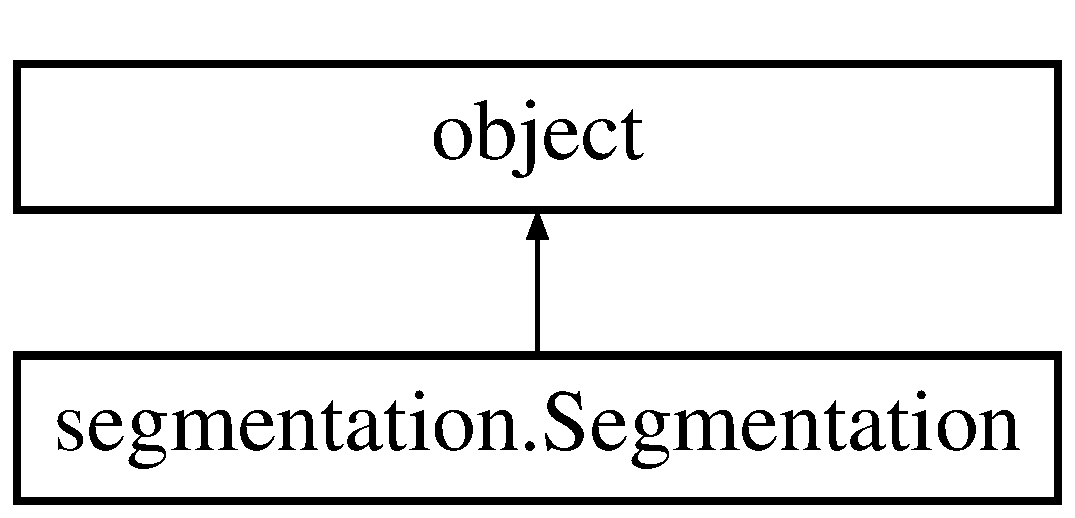
\includegraphics[height=2.000000cm]{classsegmentation_1_1_segmentation}
\end{center}
\end{figure}
\subsection*{Public Member Functions}
\begin{DoxyCompactItemize}
\item 
def \hyperlink{classsegmentation_1_1_segmentation_a1a50054187dc1e2eebe8685fdd208bf6}{\+\_\+\+\_\+init\+\_\+\+\_\+} (self, depth\+Image, pos2D)
\item 
def \hyperlink{classsegmentation_1_1_segmentation_a9ceb7a7b25953d9b693ab9f6fa1e6e3a}{find\+Slope} (self, A, B)
\item 
def \hyperlink{classsegmentation_1_1_segmentation_abc300f2410a48845de0e9ae32df38241}{infered\+Point} (self, A, a, b, c, point, T=100)
\item 
def \hyperlink{classsegmentation_1_1_segmentation_abbd3c1929edf660b23d908a99e2775ab}{polygon} (self, slopes, ref, limit)
\item 
def \hyperlink{classsegmentation_1_1_segmentation_a3fe70a2d840350c65e39d2f3938826bf}{polygon\+\_\+optimize} (self, slopes, ref, limit)
\item 
def \hyperlink{classsegmentation_1_1_segmentation_a13657232294fa4956ad7426d18ebfab4}{polygon\+Outline} (self, points)
\item 
def \hyperlink{classsegmentation_1_1_segmentation_a887e7665b0fc07dfb964223ef50dc295}{nearest\+Peak} (self, A, hip\+Left, hip\+Right, knee\+\_\+right)
\item 
def \hyperlink{classsegmentation_1_1_segmentation_acb6b057c22d3abbcc7de4e14453cfdc6}{arm\+Seg} (self, A, B, side)
\item 
def \hyperlink{classsegmentation_1_1_segmentation_a095a3b3205d784d6e7c3e072945ae7a5}{leg\+Seg} (self, A, side)
\item 
def \hyperlink{classsegmentation_1_1_segmentation_a57bb91652be301652103fa04944fced9}{head\+Seg} (self, A)
\item 
def \hyperlink{classsegmentation_1_1_segmentation_a974ac6a7e245713d6f5f2b7531fe6d71}{Get\+Body} (self, binary\+Image)
\item 
def \hyperlink{classsegmentation_1_1_segmentation_ac40379d03b4adb8c368d7d7d12e0d321}{Get\+Hand} (self, binary\+Image, side)
\item 
def \hyperlink{classsegmentation_1_1_segmentation_ad4a3e196437e4577129dc7c5aed2f559}{Get\+Foot} (self, binary\+Image, side)
\end{DoxyCompactItemize}
\subsection*{Public Attributes}
\begin{DoxyCompactItemize}
\item 
\mbox{\Hypertarget{classsegmentation_1_1_segmentation_a36ea52b517559b5691e5bc72588b2701}\label{classsegmentation_1_1_segmentation_a36ea52b517559b5691e5bc72588b2701}} 
{\bfseries depth\+Image}
\item 
\mbox{\Hypertarget{classsegmentation_1_1_segmentation_a354e16a494df339af336594c1e1844f0}\label{classsegmentation_1_1_segmentation_a354e16a494df339af336594c1e1844f0}} 
{\bfseries pos2D}
\item 
\mbox{\Hypertarget{classsegmentation_1_1_segmentation_aacd82fcfebb0f0cd30f9e45c96f6394b}\label{classsegmentation_1_1_segmentation_aacd82fcfebb0f0cd30f9e45c96f6394b}} 
{\bfseries body\+Pts}
\item 
\mbox{\Hypertarget{classsegmentation_1_1_segmentation_a7302304f2b0c3d89af45c50aa33a828c}\label{classsegmentation_1_1_segmentation_a7302304f2b0c3d89af45c50aa33a828c}} 
{\bfseries fore\+Arm\+PtsR}
\item 
\mbox{\Hypertarget{classsegmentation_1_1_segmentation_ad1a1f1e70672d02fff598618e147d0c8}\label{classsegmentation_1_1_segmentation_ad1a1f1e70672d02fff598618e147d0c8}} 
{\bfseries fore\+Arm\+PtsL}
\item 
\mbox{\Hypertarget{classsegmentation_1_1_segmentation_af82bbe5af405d55ecf4b95f9bf13f395}\label{classsegmentation_1_1_segmentation_af82bbe5af405d55ecf4b95f9bf13f395}} 
{\bfseries upper\+Arm\+PtsR}
\item 
\mbox{\Hypertarget{classsegmentation_1_1_segmentation_acd5f5a3d2af4b3132a8c47a4f74464d7}\label{classsegmentation_1_1_segmentation_acd5f5a3d2af4b3132a8c47a4f74464d7}} 
{\bfseries upper\+Arm\+PtsL}
\item 
\mbox{\Hypertarget{classsegmentation_1_1_segmentation_ab687d252753954c9d8a532e5b098e637}\label{classsegmentation_1_1_segmentation_ab687d252753954c9d8a532e5b098e637}} 
\hyperlink{classsegmentation_1_1_segmentation_ab687d252753954c9d8a532e5b098e637}{thigh\+PtsR}
\begin{DoxyCompactList}\small\item\em Find the Thigh find the fifth point that can not be deduce simply with Slopes or intersection using the entire hip. \end{DoxyCompactList}\item 
\mbox{\Hypertarget{classsegmentation_1_1_segmentation_a32dde4e5585db094b44c3ab757f3ab9e}\label{classsegmentation_1_1_segmentation_a32dde4e5585db094b44c3ab757f3ab9e}} 
{\bfseries thigh\+PtsL}
\item 
\mbox{\Hypertarget{classsegmentation_1_1_segmentation_aa926f14b37ee6275803ad15bbf417310}\label{classsegmentation_1_1_segmentation_aa926f14b37ee6275803ad15bbf417310}} 
\hyperlink{classsegmentation_1_1_segmentation_aa926f14b37ee6275803ad15bbf417310}{calf\+PtsR}
\begin{DoxyCompactList}\small\item\em Find Calf Define slopes. \end{DoxyCompactList}\item 
\mbox{\Hypertarget{classsegmentation_1_1_segmentation_a31e43c1089bb4017d23601a86c13fba7}\label{classsegmentation_1_1_segmentation_a31e43c1089bb4017d23601a86c13fba7}} 
{\bfseries calf\+PtsL}
\item 
\mbox{\Hypertarget{classsegmentation_1_1_segmentation_a560a42d6f83dfe01e32efb93fff9eecf}\label{classsegmentation_1_1_segmentation_a560a42d6f83dfe01e32efb93fff9eecf}} 
{\bfseries head\+Pts}
\end{DoxyCompactItemize}


\subsection{Detailed Description}
\begin{DoxyVerb}Segmentation process concerning body parts
\end{DoxyVerb}
 

\subsection{Constructor \& Destructor Documentation}
\mbox{\Hypertarget{classsegmentation_1_1_segmentation_a1a50054187dc1e2eebe8685fdd208bf6}\label{classsegmentation_1_1_segmentation_a1a50054187dc1e2eebe8685fdd208bf6}} 
\index{segmentation\+::\+Segmentation@{segmentation\+::\+Segmentation}!\+\_\+\+\_\+init\+\_\+\+\_\+@{\+\_\+\+\_\+init\+\_\+\+\_\+}}
\index{\+\_\+\+\_\+init\+\_\+\+\_\+@{\+\_\+\+\_\+init\+\_\+\+\_\+}!segmentation\+::\+Segmentation@{segmentation\+::\+Segmentation}}
\subsubsection{\texorpdfstring{\+\_\+\+\_\+init\+\_\+\+\_\+()}{\_\_init\_\_()}}
{\footnotesize\ttfamily def segmentation.\+Segmentation.\+\_\+\+\_\+init\+\_\+\+\_\+ (\begin{DoxyParamCaption}\item[{}]{self,  }\item[{}]{depth\+Image,  }\item[{}]{pos2D }\end{DoxyParamCaption})}

\begin{DoxyVerb}Constructor
:param depthImage: Cropped depth image of the current image
:param pos2D: list of position of the junction
\end{DoxyVerb}
 

\subsection{Member Function Documentation}
\mbox{\Hypertarget{classsegmentation_1_1_segmentation_acb6b057c22d3abbcc7de4e14453cfdc6}\label{classsegmentation_1_1_segmentation_acb6b057c22d3abbcc7de4e14453cfdc6}} 
\index{segmentation\+::\+Segmentation@{segmentation\+::\+Segmentation}!arm\+Seg@{arm\+Seg}}
\index{arm\+Seg@{arm\+Seg}!segmentation\+::\+Segmentation@{segmentation\+::\+Segmentation}}
\subsubsection{\texorpdfstring{arm\+Seg()}{armSeg()}}
{\footnotesize\ttfamily def segmentation.\+Segmentation.\+arm\+Seg (\begin{DoxyParamCaption}\item[{}]{self,  }\item[{}]{A,  }\item[{}]{B,  }\item[{}]{side }\end{DoxyParamCaption})}

\begin{DoxyVerb}Segment the left arm into two body parts
:param A: depthImag
:param B: depthImg after bilateral filtering
:param side: if side = 0 the segmentation will be done for the right arm
  otherwise it will be for the left arm
:return: an array containing two body parts : an upper arm and a lower arm
\end{DoxyVerb}
 \mbox{\Hypertarget{classsegmentation_1_1_segmentation_a9ceb7a7b25953d9b693ab9f6fa1e6e3a}\label{classsegmentation_1_1_segmentation_a9ceb7a7b25953d9b693ab9f6fa1e6e3a}} 
\index{segmentation\+::\+Segmentation@{segmentation\+::\+Segmentation}!find\+Slope@{find\+Slope}}
\index{find\+Slope@{find\+Slope}!segmentation\+::\+Segmentation@{segmentation\+::\+Segmentation}}
\subsubsection{\texorpdfstring{find\+Slope()}{findSlope()}}
{\footnotesize\ttfamily def segmentation.\+Segmentation.\+find\+Slope (\begin{DoxyParamCaption}\item[{}]{self,  }\item[{}]{A,  }\item[{}]{B }\end{DoxyParamCaption})}

\begin{DoxyVerb}Get the slope of a line made from two point A and B or the distance in one axes
:param A: point 1
:param B: point 2
:return: an array of coefficient
a is the normalized distance in the x axis
b is the normalized distance in the y axis
c is the slope between the two points
\end{DoxyVerb}
 \mbox{\Hypertarget{classsegmentation_1_1_segmentation_a974ac6a7e245713d6f5f2b7531fe6d71}\label{classsegmentation_1_1_segmentation_a974ac6a7e245713d6f5f2b7531fe6d71}} 
\index{segmentation\+::\+Segmentation@{segmentation\+::\+Segmentation}!Get\+Body@{Get\+Body}}
\index{Get\+Body@{Get\+Body}!segmentation\+::\+Segmentation@{segmentation\+::\+Segmentation}}
\subsubsection{\texorpdfstring{Get\+Body()}{GetBody()}}
{\footnotesize\ttfamily def segmentation.\+Segmentation.\+Get\+Body (\begin{DoxyParamCaption}\item[{}]{self,  }\item[{}]{binary\+Image }\end{DoxyParamCaption})}

\begin{DoxyVerb}Delete all the unwanted connected component from the binary image
It focuses on the group having the right pos2D, for now the body
:param binaryImage: binary image of the body but all body part are substracted to the body leaving only the trunck and noise
:return: trunk
\end{DoxyVerb}
 \mbox{\Hypertarget{classsegmentation_1_1_segmentation_ad4a3e196437e4577129dc7c5aed2f559}\label{classsegmentation_1_1_segmentation_ad4a3e196437e4577129dc7c5aed2f559}} 
\index{segmentation\+::\+Segmentation@{segmentation\+::\+Segmentation}!Get\+Foot@{Get\+Foot}}
\index{Get\+Foot@{Get\+Foot}!segmentation\+::\+Segmentation@{segmentation\+::\+Segmentation}}
\subsubsection{\texorpdfstring{Get\+Foot()}{GetFoot()}}
{\footnotesize\ttfamily def segmentation.\+Segmentation.\+Get\+Foot (\begin{DoxyParamCaption}\item[{}]{self,  }\item[{}]{binary\+Image,  }\item[{}]{side }\end{DoxyParamCaption})}

\begin{DoxyVerb}Delete all the little group unwanted from the binary image
It focuses on the group having the right pos2D, here the feet
:param binaryImage: binary image of the body without limbs
:param side: if side = 0 the segmentation will be done for the right feet
  otherwise it will be for the left feet
:return: one feet
\end{DoxyVerb}
 \mbox{\Hypertarget{classsegmentation_1_1_segmentation_ac40379d03b4adb8c368d7d7d12e0d321}\label{classsegmentation_1_1_segmentation_ac40379d03b4adb8c368d7d7d12e0d321}} 
\index{segmentation\+::\+Segmentation@{segmentation\+::\+Segmentation}!Get\+Hand@{Get\+Hand}}
\index{Get\+Hand@{Get\+Hand}!segmentation\+::\+Segmentation@{segmentation\+::\+Segmentation}}
\subsubsection{\texorpdfstring{Get\+Hand()}{GetHand()}}
{\footnotesize\ttfamily def segmentation.\+Segmentation.\+Get\+Hand (\begin{DoxyParamCaption}\item[{}]{self,  }\item[{}]{binary\+Image,  }\item[{}]{side }\end{DoxyParamCaption})}

\begin{DoxyVerb}Delete all the little group unwanted from the binary image
It focuses on the group having the right pos2D, here the hands
:param binaryImage: binary image of the body without limbs
:param side: if side = 0 the segmentation will be done for the right hand
  otherwise it will be for the left hand
:return: one hand
\end{DoxyVerb}
 \mbox{\Hypertarget{classsegmentation_1_1_segmentation_a57bb91652be301652103fa04944fced9}\label{classsegmentation_1_1_segmentation_a57bb91652be301652103fa04944fced9}} 
\index{segmentation\+::\+Segmentation@{segmentation\+::\+Segmentation}!head\+Seg@{head\+Seg}}
\index{head\+Seg@{head\+Seg}!segmentation\+::\+Segmentation@{segmentation\+::\+Segmentation}}
\subsubsection{\texorpdfstring{head\+Seg()}{headSeg()}}
{\footnotesize\ttfamily def segmentation.\+Segmentation.\+head\+Seg (\begin{DoxyParamCaption}\item[{}]{self,  }\item[{}]{A }\end{DoxyParamCaption})}

\begin{DoxyVerb}Segment the head
:param A: binary depthImag
:return: head body part
\end{DoxyVerb}
 \mbox{\Hypertarget{classsegmentation_1_1_segmentation_abc300f2410a48845de0e9ae32df38241}\label{classsegmentation_1_1_segmentation_abc300f2410a48845de0e9ae32df38241}} 
\index{segmentation\+::\+Segmentation@{segmentation\+::\+Segmentation}!infered\+Point@{infered\+Point}}
\index{infered\+Point@{infered\+Point}!segmentation\+::\+Segmentation@{segmentation\+::\+Segmentation}}
\subsubsection{\texorpdfstring{infered\+Point()}{inferedPoint()}}
{\footnotesize\ttfamily def segmentation.\+Segmentation.\+infered\+Point (\begin{DoxyParamCaption}\item[{}]{self,  }\item[{}]{A,  }\item[{}]{a,  }\item[{}]{b,  }\item[{}]{c,  }\item[{}]{point,  }\item[{}]{T = {\ttfamily 100} }\end{DoxyParamCaption})}

\begin{DoxyVerb}Find two points that are the corners of the segmented part
:param A: Depth Image
:param a: dist x axe between two points
:param b: dist y axe between two points
:param c: slope between two points
:param point: a junction
:param T: max distance to find intersection
:return: two intersection points between a slope and the edges of the body part
\end{DoxyVerb}
 \mbox{\Hypertarget{classsegmentation_1_1_segmentation_a095a3b3205d784d6e7c3e072945ae7a5}\label{classsegmentation_1_1_segmentation_a095a3b3205d784d6e7c3e072945ae7a5}} 
\index{segmentation\+::\+Segmentation@{segmentation\+::\+Segmentation}!leg\+Seg@{leg\+Seg}}
\index{leg\+Seg@{leg\+Seg}!segmentation\+::\+Segmentation@{segmentation\+::\+Segmentation}}
\subsubsection{\texorpdfstring{leg\+Seg()}{legSeg()}}
{\footnotesize\ttfamily def segmentation.\+Segmentation.\+leg\+Seg (\begin{DoxyParamCaption}\item[{}]{self,  }\item[{}]{A,  }\item[{}]{side }\end{DoxyParamCaption})}

\begin{DoxyVerb}Segment the leg into two body parts
:param A: depthImag
:param side: if side = 0 the segmentation will be done for the right leg
  otherwise it will be for the left leg
:return: an array containing two body parts : an upper leg and a lower leg
\end{DoxyVerb}
 \mbox{\Hypertarget{classsegmentation_1_1_segmentation_a887e7665b0fc07dfb964223ef50dc295}\label{classsegmentation_1_1_segmentation_a887e7665b0fc07dfb964223ef50dc295}} 
\index{segmentation\+::\+Segmentation@{segmentation\+::\+Segmentation}!nearest\+Peak@{nearest\+Peak}}
\index{nearest\+Peak@{nearest\+Peak}!segmentation\+::\+Segmentation@{segmentation\+::\+Segmentation}}
\subsubsection{\texorpdfstring{nearest\+Peak()}{nearestPeak()}}
{\footnotesize\ttfamily def segmentation.\+Segmentation.\+nearest\+Peak (\begin{DoxyParamCaption}\item[{}]{self,  }\item[{}]{A,  }\item[{}]{hip\+Left,  }\item[{}]{hip\+Right,  }\item[{}]{knee\+\_\+right }\end{DoxyParamCaption})}

\begin{DoxyVerb}In the case of upper legs, find the point in between the two upper legs that is at a edge of the hip
:param A: binary image
:param hipLeft: left hip junctions
:param hipRight:  right hip junctions
:param knee_right: right knee junctions
:return: return a point at the edge and between the two legs
Make drawing will help to understand
\end{DoxyVerb}
 \mbox{\Hypertarget{classsegmentation_1_1_segmentation_abbd3c1929edf660b23d908a99e2775ab}\label{classsegmentation_1_1_segmentation_abbd3c1929edf660b23d908a99e2775ab}} 
\index{segmentation\+::\+Segmentation@{segmentation\+::\+Segmentation}!polygon@{polygon}}
\index{polygon@{polygon}!segmentation\+::\+Segmentation@{segmentation\+::\+Segmentation}}
\subsubsection{\texorpdfstring{polygon()}{polygon()}}
{\footnotesize\ttfamily def segmentation.\+Segmentation.\+polygon (\begin{DoxyParamCaption}\item[{}]{self,  }\item[{}]{slopes,  }\item[{}]{ref,  }\item[{}]{limit }\end{DoxyParamCaption})}

\begin{DoxyVerb}Test the sign of alpha = (a[k]*j+b[k]*i+c[k])*ref[k]
to know whether a point is within a polygon or not
:param slopes: list of slopes defining a the border lines of the polygone
:param ref:  a point inside the polygon
:param limit: number of slopes
:return: the body part filled with true.
\end{DoxyVerb}
 \mbox{\Hypertarget{classsegmentation_1_1_segmentation_a3fe70a2d840350c65e39d2f3938826bf}\label{classsegmentation_1_1_segmentation_a3fe70a2d840350c65e39d2f3938826bf}} 
\index{segmentation\+::\+Segmentation@{segmentation\+::\+Segmentation}!polygon\+\_\+optimize@{polygon\+\_\+optimize}}
\index{polygon\+\_\+optimize@{polygon\+\_\+optimize}!segmentation\+::\+Segmentation@{segmentation\+::\+Segmentation}}
\subsubsection{\texorpdfstring{polygon\+\_\+optimize()}{polygon\_optimize()}}
{\footnotesize\ttfamily def segmentation.\+Segmentation.\+polygon\+\_\+optimize (\begin{DoxyParamCaption}\item[{}]{self,  }\item[{}]{slopes,  }\item[{}]{ref,  }\item[{}]{limit }\end{DoxyParamCaption})}

\begin{DoxyVerb}Test the sign of alpha = (a[k]*j+b[k]*i+c[k])*ref[k]
to know whether a point is within a polygon or not
:param slopes: list of slopes defining a the border lines of the polygone
:param ref:  a point inside the polygon
:param limit: number of slopes
:return: the body part filled with true.
\end{DoxyVerb}
 \mbox{\Hypertarget{classsegmentation_1_1_segmentation_a13657232294fa4956ad7426d18ebfab4}\label{classsegmentation_1_1_segmentation_a13657232294fa4956ad7426d18ebfab4}} 
\index{segmentation\+::\+Segmentation@{segmentation\+::\+Segmentation}!polygon\+Outline@{polygon\+Outline}}
\index{polygon\+Outline@{polygon\+Outline}!segmentation\+::\+Segmentation@{segmentation\+::\+Segmentation}}
\subsubsection{\texorpdfstring{polygon\+Outline()}{polygonOutline()}}
{\footnotesize\ttfamily def segmentation.\+Segmentation.\+polygon\+Outline (\begin{DoxyParamCaption}\item[{}]{self,  }\item[{}]{points }\end{DoxyParamCaption})}

\begin{DoxyVerb}Find a polygon on the image through the points given in points
:param points: array of points which are the corners of the polygon to find
:return:  the body part filled with true.
\end{DoxyVerb}
 

The documentation for this class was generated from the following file\+:\begin{DoxyCompactItemize}
\item 
code/lib/segmentation.\+py\end{DoxyCompactItemize}

\section{Stitching.\+Stitch Class Reference}
\label{class_stitching_1_1_stitch}\index{Stitching.\+Stitch@{Stitching.\+Stitch}}
\subsection*{Public Member Functions}
\begin{DoxyCompactItemize}
\item 
def \textbf{ \+\_\+\+\_\+init\+\_\+\+\_\+} (self, number\+\_\+body\+Part)
\item 
def \textbf{ Naive\+Stitch} (self, Part\+Vtx, Part\+Nmls, Part\+Faces, Pose\+BP)
\item 
def \textbf{ Transform\+Vtx} (self, Vtx, Pose, s)
\item 
def \textbf{ Transform\+Nmls} (self, Nmls, Pose, s)
\item 
def \textbf{ R\+Arms\+Transform} (self, angle, bp, pos2d, R\+G\+BD, Tg)
\item 
def \textbf{ Get\+B\+B\+Transfo} (self, pos2d, cur, prev, R\+G\+BD, bp)
\item 
def \textbf{ Get\+Coord\+Syst} (self, pos2d, jt, R\+G\+BD, bp)
\item 
def \textbf{ Get\+Pos} (self, bp)
\end{DoxyCompactItemize}
\subsection*{Public Attributes}
\begin{DoxyCompactItemize}
\item 
\mbox{\label{class_stitching_1_1_stitch_a6984b78515332ecfd8c9bfd783f91e49}} 
{\bfseries nb\+\_\+bp}
\item 
\mbox{\label{class_stitching_1_1_stitch_a4de61586c9c27338b95e1a0ccefc3c34}} 
{\bfseries Stitched\+Vertices}
\item 
\mbox{\label{class_stitching_1_1_stitch_ad76a66008928b460d7c1b7e82972cbeb}} 
{\bfseries Stitched\+Faces}
\item 
\mbox{\label{class_stitching_1_1_stitch_a4744a49d727d4966433272eb4f721560}} 
{\bfseries Stitched\+Normales}
\end{DoxyCompactItemize}


\subsection{Detailed Description}
\begin{DoxyVerb}All method that concern linking or aligning body parts together are in Stitch
\end{DoxyVerb}
 

\subsection{Constructor \& Destructor Documentation}
\mbox{\label{class_stitching_1_1_stitch_ab891a54caf4e40cd3a6eacdfae3d08f2}} 
\index{Stitching\+::\+Stitch@{Stitching\+::\+Stitch}!\+\_\+\+\_\+init\+\_\+\+\_\+@{\+\_\+\+\_\+init\+\_\+\+\_\+}}
\index{\+\_\+\+\_\+init\+\_\+\+\_\+@{\+\_\+\+\_\+init\+\_\+\+\_\+}!Stitching\+::\+Stitch@{Stitching\+::\+Stitch}}
\subsubsection{\+\_\+\+\_\+init\+\_\+\+\_\+()}
{\footnotesize\ttfamily def Stitching.\+Stitch.\+\_\+\+\_\+init\+\_\+\+\_\+ (\begin{DoxyParamCaption}\item[{}]{self,  }\item[{}]{number\+\_\+body\+Part }\end{DoxyParamCaption})}

\begin{DoxyVerb}Constructor
:param number_bodyPart: number of body parts
\end{DoxyVerb}
 

\subsection{Member Function Documentation}
\mbox{\label{class_stitching_1_1_stitch_a24d4c32a258141cbdc3cfa3bae127fe7}} 
\index{Stitching\+::\+Stitch@{Stitching\+::\+Stitch}!Get\+B\+B\+Transfo@{Get\+B\+B\+Transfo}}
\index{Get\+B\+B\+Transfo@{Get\+B\+B\+Transfo}!Stitching\+::\+Stitch@{Stitching\+::\+Stitch}}
\subsubsection{Get\+B\+B\+Transfo()}
{\footnotesize\ttfamily def Stitching.\+Stitch.\+Get\+B\+B\+Transfo (\begin{DoxyParamCaption}\item[{}]{self,  }\item[{}]{pos2d,  }\item[{}]{cur,  }\item[{}]{prev,  }\item[{}]{R\+G\+BD,  }\item[{}]{bp }\end{DoxyParamCaption})}

\begin{DoxyVerb}Transform Pose matrix to move the model body parts according to the position of the skeleton
For now just a rotation in the z axis
:param bp : number of the body parts
:param pos2d : position in 2D of the junctions
:param cur : index for the current frame
:param prev : index for the previous frame
:param RGBD : an RGBD object containing the image
:return The transform between two skeleton
\end{DoxyVerb}
 \mbox{\label{class_stitching_1_1_stitch_ae2a91306c029bcd2b6631a64d662cbff}} 
\index{Stitching\+::\+Stitch@{Stitching\+::\+Stitch}!Get\+Coord\+Syst@{Get\+Coord\+Syst}}
\index{Get\+Coord\+Syst@{Get\+Coord\+Syst}!Stitching\+::\+Stitch@{Stitching\+::\+Stitch}}
\subsubsection{Get\+Coord\+Syst()}
{\footnotesize\ttfamily def Stitching.\+Stitch.\+Get\+Coord\+Syst (\begin{DoxyParamCaption}\item[{}]{self,  }\item[{}]{pos2d,  }\item[{}]{jt,  }\item[{}]{R\+G\+BD,  }\item[{}]{bp }\end{DoxyParamCaption})}

\begin{DoxyVerb}This function compute the coordinates system of a body part according to the camera pose
:param pos2d: camera pose
:param jt: junctions of the body parts
:param RGBD: Image
:param bp: number of body part
:return: Matrix containing the coordinates systems
\end{DoxyVerb}
 \mbox{\label{class_stitching_1_1_stitch_a0ba4c013f984b9b0fa636a2d120094d2}} 
\index{Stitching\+::\+Stitch@{Stitching\+::\+Stitch}!Get\+Pos@{Get\+Pos}}
\index{Get\+Pos@{Get\+Pos}!Stitching\+::\+Stitch@{Stitching\+::\+Stitch}}
\subsubsection{Get\+Pos()}
{\footnotesize\ttfamily def Stitching.\+Stitch.\+Get\+Pos (\begin{DoxyParamCaption}\item[{}]{self,  }\item[{}]{bp }\end{DoxyParamCaption})}

\begin{DoxyVerb}According to the body parts, get the correct index of junctions
mid is used to get the center while pos1 and pos2 give extremes junctions of the body parts
:param bp: number of the body part
:return: return the junctions corresponding to the body parts
\end{DoxyVerb}
 \mbox{\label{class_stitching_1_1_stitch_ac88004e122bb16c19ef3038d856be04a}} 
\index{Stitching\+::\+Stitch@{Stitching\+::\+Stitch}!Naive\+Stitch@{Naive\+Stitch}}
\index{Naive\+Stitch@{Naive\+Stitch}!Stitching\+::\+Stitch@{Stitching\+::\+Stitch}}
\subsubsection{Naive\+Stitch()}
{\footnotesize\ttfamily def Stitching.\+Stitch.\+Naive\+Stitch (\begin{DoxyParamCaption}\item[{}]{self,  }\item[{}]{Part\+Vtx,  }\item[{}]{Part\+Nmls,  }\item[{}]{Part\+Faces,  }\item[{}]{Pose\+BP }\end{DoxyParamCaption})}

\begin{DoxyVerb}Add the vertices and faces of each body parts
together after transforming them in the global coordinates system
:param PartVtx: List of vertices for a body parts
:param PartNmls: List of normales for a body parts
:param PartFaces:  List of faces for a body parts
:param PoseBP: local to global transform
:return: none
\end{DoxyVerb}
 \mbox{\label{class_stitching_1_1_stitch_a14624518ed5cbc4422762ff59d3c5bb8}} 
\index{Stitching\+::\+Stitch@{Stitching\+::\+Stitch}!R\+Arms\+Transform@{R\+Arms\+Transform}}
\index{R\+Arms\+Transform@{R\+Arms\+Transform}!Stitching\+::\+Stitch@{Stitching\+::\+Stitch}}
\subsubsection{R\+Arms\+Transform()}
{\footnotesize\ttfamily def Stitching.\+Stitch.\+R\+Arms\+Transform (\begin{DoxyParamCaption}\item[{}]{self,  }\item[{}]{angle,  }\item[{}]{bp,  }\item[{}]{pos2d,  }\item[{}]{R\+G\+BD,  }\item[{}]{Tg }\end{DoxyParamCaption})}

\begin{DoxyVerb}Transform Pose matrix to move the model of the right arm
For now just a rotation in the z axis
:param bp : number of the body parts
:param pos2d : position in 2D of the junctions
:param RGBD : an RGBD object containing the image
:param Tg : local to global transform
TEST FUNCTION : TURN THE LEFT ARM OF THE SEGMENTED BODY.
\end{DoxyVerb}
 \mbox{\label{class_stitching_1_1_stitch_a9df52cb70ec0a02cf93ac0ea9f09706c}} 
\index{Stitching\+::\+Stitch@{Stitching\+::\+Stitch}!Transform\+Nmls@{Transform\+Nmls}}
\index{Transform\+Nmls@{Transform\+Nmls}!Stitching\+::\+Stitch@{Stitching\+::\+Stitch}}
\subsubsection{Transform\+Nmls()}
{\footnotesize\ttfamily def Stitching.\+Stitch.\+Transform\+Nmls (\begin{DoxyParamCaption}\item[{}]{self,  }\item[{}]{Nmls,  }\item[{}]{Pose,  }\item[{}]{s }\end{DoxyParamCaption})}

\begin{DoxyVerb}Transform the normales in a system to another system.
Here it will be mostly used to transform from local system to global coordiantes system
:param Nmls:  List of normales
:param Pose: local to global transform
:param s: subsampling factor
:return: list of transformed normales
\end{DoxyVerb}
 \mbox{\label{class_stitching_1_1_stitch_addf2733c95c1a99895485f639989c971}} 
\index{Stitching\+::\+Stitch@{Stitching\+::\+Stitch}!Transform\+Vtx@{Transform\+Vtx}}
\index{Transform\+Vtx@{Transform\+Vtx}!Stitching\+::\+Stitch@{Stitching\+::\+Stitch}}
\subsubsection{Transform\+Vtx()}
{\footnotesize\ttfamily def Stitching.\+Stitch.\+Transform\+Vtx (\begin{DoxyParamCaption}\item[{}]{self,  }\item[{}]{Vtx,  }\item[{}]{Pose,  }\item[{}]{s }\end{DoxyParamCaption})}

\begin{DoxyVerb}Transform the vertices in a system to another system.
Here it will be mostly used to transform from local system to global coordiantes system
:param Vtx: List of vertices
:param Pose:  local to global transform
:param s: subsampling factor
:return: list of transformed vertices
\end{DoxyVerb}
 

The documentation for this class was generated from the following file\+:\begin{DoxyCompactItemize}
\item 
lib/Stitching.\+py\end{DoxyCompactItemize}

\hypertarget{classtracking_1_1_tracker}{}\section{tracking.\+Tracker Class Reference}
\label{classtracking_1_1_tracker}\index{tracking.\+Tracker@{tracking.\+Tracker}}
\subsection*{Public Member Functions}
\begin{DoxyCompactItemize}
\item 
def \hyperlink{classtracking_1_1_tracker_af4ec0591320a6a3186198e4afa34aa4a}{\+\_\+\+\_\+init\+\_\+\+\_\+} (self, thresh\+\_\+dist, thresh\+\_\+norm, lvl, max\+\_\+iter)
\item 
def \hyperlink{classtracking_1_1_tracker_a74ff598370a1334ee1cf35a1d8c3c5b8}{Register\+R\+G\+BD} (self, Image1, Image2)
\item 
def \hyperlink{classtracking_1_1_tracker_a67305bad91e92f81957982b6b92556cc}{Register\+R\+G\+B\+D\+\_\+optimize} (self, Image1, Image2)
\item 
def \hyperlink{classtracking_1_1_tracker_a99da5721b34cdb54cf89534ab2a77f35}{Register\+R\+G\+B\+D\+Mesh} (self, New\+Image, Mesh\+Vtx, Mesh\+Nmls, Pose)
\item 
def \hyperlink{classtracking_1_1_tracker_a435754ca561996d43da1bd5d91b9ad36}{Register\+R\+G\+B\+D\+Mesh\+\_\+optimize} (self, New\+Image, Mesh\+Vtx, Mesh\+Nmls, Pose)
\end{DoxyCompactItemize}
\subsection*{Public Attributes}
\begin{DoxyCompactItemize}
\item 
\mbox{\Hypertarget{classtracking_1_1_tracker_a1f46d5b2dae7afdaa90a82c9c9105f44}\label{classtracking_1_1_tracker_a1f46d5b2dae7afdaa90a82c9c9105f44}} 
{\bfseries thresh\+\_\+dist}
\item 
\mbox{\Hypertarget{classtracking_1_1_tracker_acfd351ce92170c6fe1f5627412ca3a6b}\label{classtracking_1_1_tracker_acfd351ce92170c6fe1f5627412ca3a6b}} 
{\bfseries thresh\+\_\+norm}
\item 
\mbox{\Hypertarget{classtracking_1_1_tracker_a08950fc3a5d4f62953bb2c5ee5f8cb16}\label{classtracking_1_1_tracker_a08950fc3a5d4f62953bb2c5ee5f8cb16}} 
{\bfseries lvl}
\item 
\mbox{\Hypertarget{classtracking_1_1_tracker_afa1bc9948ab57bffca4ea0fb99a324de}\label{classtracking_1_1_tracker_afa1bc9948ab57bffca4ea0fb99a324de}} 
{\bfseries max\+\_\+iter}
\end{DoxyCompactItemize}


\subsection{Detailed Description}
\begin{DoxyVerb}Tracking camera pose class
\end{DoxyVerb}
 

\subsection{Constructor \& Destructor Documentation}
\mbox{\Hypertarget{classtracking_1_1_tracker_af4ec0591320a6a3186198e4afa34aa4a}\label{classtracking_1_1_tracker_af4ec0591320a6a3186198e4afa34aa4a}} 
\index{tracking\+::\+Tracker@{tracking\+::\+Tracker}!\+\_\+\+\_\+init\+\_\+\+\_\+@{\+\_\+\+\_\+init\+\_\+\+\_\+}}
\index{\+\_\+\+\_\+init\+\_\+\+\_\+@{\+\_\+\+\_\+init\+\_\+\+\_\+}!tracking\+::\+Tracker@{tracking\+::\+Tracker}}
\subsubsection{\texorpdfstring{\+\_\+\+\_\+init\+\_\+\+\_\+()}{\_\_init\_\_()}}
{\footnotesize\ttfamily def tracking.\+Tracker.\+\_\+\+\_\+init\+\_\+\+\_\+ (\begin{DoxyParamCaption}\item[{}]{self,  }\item[{}]{thresh\+\_\+dist,  }\item[{}]{thresh\+\_\+norm,  }\item[{}]{lvl,  }\item[{}]{max\+\_\+iter }\end{DoxyParamCaption})}

\begin{DoxyVerb}Constructor
:param thresh_dist: threshold for distance between vertices
:param thresh_norm: threshold for distance between normales
:param lvl:
:param max_iter: maximum number of iteration
\end{DoxyVerb}
 

\subsection{Member Function Documentation}
\mbox{\Hypertarget{classtracking_1_1_tracker_a74ff598370a1334ee1cf35a1d8c3c5b8}\label{classtracking_1_1_tracker_a74ff598370a1334ee1cf35a1d8c3c5b8}} 
\index{tracking\+::\+Tracker@{tracking\+::\+Tracker}!Register\+R\+G\+BD@{Register\+R\+G\+BD}}
\index{Register\+R\+G\+BD@{Register\+R\+G\+BD}!tracking\+::\+Tracker@{tracking\+::\+Tracker}}
\subsubsection{\texorpdfstring{Register\+R\+G\+B\+D()}{RegisterRGBD()}}
{\footnotesize\ttfamily def tracking.\+Tracker.\+Register\+R\+G\+BD (\begin{DoxyParamCaption}\item[{}]{self,  }\item[{}]{Image1,  }\item[{}]{Image2 }\end{DoxyParamCaption})}

\begin{DoxyVerb}Function that estimate the relative rigid transformation between two input RGB-D images
:param Image1: First RGBD images
:param Image2:  Second RGBD images
:return: Transform matrix between Image1 and Image2
\end{DoxyVerb}
 \mbox{\Hypertarget{classtracking_1_1_tracker_a67305bad91e92f81957982b6b92556cc}\label{classtracking_1_1_tracker_a67305bad91e92f81957982b6b92556cc}} 
\index{tracking\+::\+Tracker@{tracking\+::\+Tracker}!Register\+R\+G\+B\+D\+\_\+optimize@{Register\+R\+G\+B\+D\+\_\+optimize}}
\index{Register\+R\+G\+B\+D\+\_\+optimize@{Register\+R\+G\+B\+D\+\_\+optimize}!tracking\+::\+Tracker@{tracking\+::\+Tracker}}
\subsubsection{\texorpdfstring{Register\+R\+G\+B\+D\+\_\+optimize()}{RegisterRGBD\_optimize()}}
{\footnotesize\ttfamily def tracking.\+Tracker.\+Register\+R\+G\+B\+D\+\_\+optimize (\begin{DoxyParamCaption}\item[{}]{self,  }\item[{}]{Image1,  }\item[{}]{Image2 }\end{DoxyParamCaption})}

\begin{DoxyVerb}Optimize version of  RegisterRGBD
:param Image1: First RGBD images
:param Image2:  Second RGBD images
:return: Transform matrix between Image1 and Image2
\end{DoxyVerb}
 \mbox{\Hypertarget{classtracking_1_1_tracker_a99da5721b34cdb54cf89534ab2a77f35}\label{classtracking_1_1_tracker_a99da5721b34cdb54cf89534ab2a77f35}} 
\index{tracking\+::\+Tracker@{tracking\+::\+Tracker}!Register\+R\+G\+B\+D\+Mesh@{Register\+R\+G\+B\+D\+Mesh}}
\index{Register\+R\+G\+B\+D\+Mesh@{Register\+R\+G\+B\+D\+Mesh}!tracking\+::\+Tracker@{tracking\+::\+Tracker}}
\subsubsection{\texorpdfstring{Register\+R\+G\+B\+D\+Mesh()}{RegisterRGBDMesh()}}
{\footnotesize\ttfamily def tracking.\+Tracker.\+Register\+R\+G\+B\+D\+Mesh (\begin{DoxyParamCaption}\item[{}]{self,  }\item[{}]{New\+Image,  }\item[{}]{Mesh\+Vtx,  }\item[{}]{Mesh\+Nmls,  }\item[{}]{Pose }\end{DoxyParamCaption})}

\begin{DoxyVerb}Function that estimate the relative rigid transformation between an input RGB-D images and a mesh
:param NewImage: RGBD image
:param MeshVtx: list of vertices of the mesh
:param MeshNmls: list of normales of the mesh
:param Pose:  estimate of the pose of the current image
:return: Transform matrix between Image1 and the mesh (transform from the first frame to the current frame)
\end{DoxyVerb}
 \mbox{\Hypertarget{classtracking_1_1_tracker_a435754ca561996d43da1bd5d91b9ad36}\label{classtracking_1_1_tracker_a435754ca561996d43da1bd5d91b9ad36}} 
\index{tracking\+::\+Tracker@{tracking\+::\+Tracker}!Register\+R\+G\+B\+D\+Mesh\+\_\+optimize@{Register\+R\+G\+B\+D\+Mesh\+\_\+optimize}}
\index{Register\+R\+G\+B\+D\+Mesh\+\_\+optimize@{Register\+R\+G\+B\+D\+Mesh\+\_\+optimize}!tracking\+::\+Tracker@{tracking\+::\+Tracker}}
\subsubsection{\texorpdfstring{Register\+R\+G\+B\+D\+Mesh\+\_\+optimize()}{RegisterRGBDMesh\_optimize()}}
{\footnotesize\ttfamily def tracking.\+Tracker.\+Register\+R\+G\+B\+D\+Mesh\+\_\+optimize (\begin{DoxyParamCaption}\item[{}]{self,  }\item[{}]{New\+Image,  }\item[{}]{Mesh\+Vtx,  }\item[{}]{Mesh\+Nmls,  }\item[{}]{Pose }\end{DoxyParamCaption})}

\begin{DoxyVerb}Optimize version with CPU  of RegisterRGBDMesh
:param NewImage: RGBD image
:param MeshVtx: list of vertices of the mesh
:param MeshNmls: list of normales of the mesh
:param Pose:  estimate of the pose of the current image
:return: Transform matrix between Image1 and the mesh (transform from the first frame to the current frame)
\end{DoxyVerb}
 

The documentation for this class was generated from the following file\+:\begin{DoxyCompactItemize}
\item 
code/lib/tracking.\+py\end{DoxyCompactItemize}

\section{T\+S\+D\+F.\+T\+S\+D\+F\+Manager Class Reference}
\label{class_t_s_d_f_1_1_t_s_d_f_manager}\index{T\+S\+D\+F.\+T\+S\+D\+F\+Manager@{T\+S\+D\+F.\+T\+S\+D\+F\+Manager}}
\subsection*{Public Member Functions}
\begin{DoxyCompactItemize}
\item 
def \textbf{ \+\_\+\+\_\+init\+\_\+\+\_\+} (self, Size, Image, G\+P\+U\+Manager)
\end{DoxyCompactItemize}
\subsection*{Public Attributes}
\begin{DoxyCompactItemize}
\item 
\mbox{\label{class_t_s_d_f_1_1_t_s_d_f_manager_a543ea4e048d1df7380bd79be3ac9dfe9}} 
{\bfseries Size}
\item 
\mbox{\label{class_t_s_d_f_1_1_t_s_d_f_manager_a5b46a7ab63020c4bbce4931609498b8c}} 
{\bfseries c\+\_\+x}
\item 
\mbox{\label{class_t_s_d_f_1_1_t_s_d_f_manager_a7edafc4388aa84442f045f2fa5b94eb8}} 
{\bfseries c\+\_\+y}
\item 
\mbox{\label{class_t_s_d_f_1_1_t_s_d_f_manager_aeba74b0bd80bc40201645176c12fe3fa}} 
{\bfseries c\+\_\+z}
\item 
\mbox{\label{class_t_s_d_f_1_1_t_s_d_f_manager_a80f1ca599244e81bd8064bf70ff715b7}} 
{\bfseries dim\+\_\+x}
\item 
\mbox{\label{class_t_s_d_f_1_1_t_s_d_f_manager_a18e227b86241c0c646d59ee8529f543b}} 
{\bfseries dim\+\_\+y}
\item 
\mbox{\label{class_t_s_d_f_1_1_t_s_d_f_manager_a8114fea25e1d0c8fb302a0facb5d2cb9}} 
{\bfseries dim\+\_\+z}
\item 
\mbox{\label{class_t_s_d_f_1_1_t_s_d_f_manager_aca3634ddaa2b18e2712cef7f974104b5}} 
{\bfseries res}
\item 
\mbox{\label{class_t_s_d_f_1_1_t_s_d_f_manager_a0dcb7c08d94a16ff39b221317c36be25}} 
{\bfseries G\+P\+U\+Manager}
\item 
\mbox{\label{class_t_s_d_f_1_1_t_s_d_f_manager_a6114aa1de6ab9d14115e514fe7f442de}} 
{\bfseries Size\+\_\+\+Volume}
\item 
\mbox{\label{class_t_s_d_f_1_1_t_s_d_f_manager_ae4a4044d7a75f29253c881a6251a9a56}} 
{\bfseries T\+S\+DF}
\item 
\mbox{\label{class_t_s_d_f_1_1_t_s_d_f_manager_a45f195df89365375e90764ec5f4db45a}} 
{\bfseries T\+S\+D\+F\+G\+PU}
\item 
\mbox{\label{class_t_s_d_f_1_1_t_s_d_f_manager_a483b831ae3d1db5673c8a52bfbfb8122}} 
{\bfseries Weight}
\item 
\mbox{\label{class_t_s_d_f_1_1_t_s_d_f_manager_a2c8e6ea973970a12c53a1c2f5c41ee3d}} 
{\bfseries Weight\+G\+PU}
\item 
\mbox{\label{class_t_s_d_f_1_1_t_s_d_f_manager_a5bd5a67350759d1753c68f4a9de7173b}} 
{\bfseries Param}
\item 
\mbox{\label{class_t_s_d_f_1_1_t_s_d_f_manager_a3ce2a5f73dbea97591620ba0a6be2cf3}} 
{\bfseries Pose}
\item 
\mbox{\label{class_t_s_d_f_1_1_t_s_d_f_manager_a0fa22055c7f9ee209143a1e20765af2b}} 
{\bfseries Depth\+G\+PU}
\item 
\mbox{\label{class_t_s_d_f_1_1_t_s_d_f_manager_a003face100e7ed90b22085c72b7cd8f1}} 
{\bfseries Calib\+\_\+\+G\+PU}
\item 
\mbox{\label{class_t_s_d_f_1_1_t_s_d_f_manager_a007719dcd94065704861fbdf742b08be}} 
{\bfseries Pose\+\_\+\+G\+PU}
\end{DoxyCompactItemize}


\subsection{Detailed Description}
\begin{DoxyVerb}Manager Truncated Signed Distance Function.
\end{DoxyVerb}
 

\subsection{Constructor \& Destructor Documentation}
\mbox{\label{class_t_s_d_f_1_1_t_s_d_f_manager_aa12aee58f9d79032e2ff5256a1eaba35}} 
\index{T\+S\+D\+F\+::\+T\+S\+D\+F\+Manager@{T\+S\+D\+F\+::\+T\+S\+D\+F\+Manager}!\+\_\+\+\_\+init\+\_\+\+\_\+@{\+\_\+\+\_\+init\+\_\+\+\_\+}}
\index{\+\_\+\+\_\+init\+\_\+\+\_\+@{\+\_\+\+\_\+init\+\_\+\+\_\+}!T\+S\+D\+F\+::\+T\+S\+D\+F\+Manager@{T\+S\+D\+F\+::\+T\+S\+D\+F\+Manager}}
\subsubsection{\+\_\+\+\_\+init\+\_\+\+\_\+()}
{\footnotesize\ttfamily def T\+S\+D\+F.\+T\+S\+D\+F\+Manager.\+\_\+\+\_\+init\+\_\+\+\_\+ (\begin{DoxyParamCaption}\item[{}]{self,  }\item[{}]{Size,  }\item[{}]{Image,  }\item[{}]{G\+P\+U\+Manager }\end{DoxyParamCaption})}

\begin{DoxyVerb}Constructor
:param Size: dimension of each axis of the volume
:param Image: RGBD image to compare
:param GPUManager: GPU environment for GPU computation
\end{DoxyVerb}
 

The documentation for this class was generated from the following file\+:\begin{DoxyCompactItemize}
\item 
lib/T\+S\+D\+F.\+py\end{DoxyCompactItemize}

%--- End generated contents ---

% Index
\backmatter
\newpage
\phantomsection
\clearemptydoublepage
\addcontentsline{toc}{chapter}{Index}
\printindex

\end{document}
